% =====================================
% %%%%%%%%%%%%%%%%%%%%%%%%%%%%%%%%%%%%
% Setup
% %%%%%%%%%%%%%%%%%%%%%%%%%%%%%%%%%%%%
% =====================================
\documentclass[letterpaper,11pt]{book}

%%%%%%%%%%%%%%%%%%%%%%%%%%
% Main Utilities:
%%%%%%%%%%%%%%%%%%%%%%%%%%
% Preamble for physics-paper-related packages and commands

% ========================
% Main packages
% ========================
\usepackage[utf8]{inputenc}

\usepackage{mathtools,amssymb,amsmath,amsthm,mathrsfs}
\usepackage{physics}
\usepackage{enumitem}
\usepackage{etoolbox}
\usepackage{yhmath}
\usepackage{changepage}


% =====================================
% Hyperlinks
% =====================================
\usepackage[hidelinks]{hyperref}

% ---------------------------------
% hyperref fixes
% ---------------------------------
% Sometimes hyperref will lead to problems, and these are some fixes:

% - - - - - - - - - - - - - - - - -
% Conflicts with \MakeUppercase
% https://tex.stackexchange.com/a/598876
% - - - - - - - - - - - - - - - - -
\def\MakeUppercaseUnsupportedInPdfStrings{\scshape}

% - - - - - - - - - - - - - - - - -
% Conflicts with... label?
% https://tex.stackexchange.com/a/130323
% - - - - - - - - - - - - - - - - -
\newcounter{numrel}% Counter for numering relations
\newcounter{Hnumrel}% Keep hyperref happy and don't duplicate anchors
\renewcommand{\thenumrel}{\roman{numrel}}% Counter numrel uses lowercase roman numerals

\makeatletter
\newcommand{\numrel}[2]{% Relation numbering
  \refstepcounter{numrel}% Increment numrel counter and create correct reference hook
  \stepcounter{Hnumrel}%
  \ifmeasuring@\else\ltx@label{#2}\fi % Label numrel counter (issue only once)
  \overset{\text{(\thenumrel)}}{#1}% Print counter + relation
}
\makeatother
\AfterEndEnvironment{align*}{\setcounter{numrel}{0}}% Resets numrel at the end of align*
% - - - - - - - - - - - - - - - - -


% ---------------------------------
% hyperref dummy functions
% ---------------------------------
% Adding dummy versions of hyperref tools to avoid errors if hyperref is _not_ used
\providecommand\phantomsection{}
\providecommand\theHfigure{}


% =====================================
% Glossary
% =====================================
% See https://en.wikibooks.org/wiki/LaTeX/Glossary
% Note: glossaries must be loaded after hyperref

% \usepackage[acronym,automake=immediate,nonumberlist,toc,xindy]{glossaries}
% \usepackage[acronym,nomain,toc,automake]{glossaries-extra}
% \usepackage[acronym,automake,toc,xindy]{glossaries-extra}
% \usepackage[acronym,automake,toc]{glossaries-extra}

\usepackage[
 % automake,% create glossaries automatically
 acronym,% create 'abbreviations' glossary
 % index,% create 'index' glossary
 nostyles,%don't load predefined styles
 % postdot,% insert dot after descriptions
 % record,% using bib2gls
 stylemods={tree,bookindex},% load the 'tree' and 'bookindex' style packages
 style={tree},% set the default style to 'tree'
 toc% add glossaries to table of contents
]{glossaries-extra}


% ---------------------------------
% Preparing for use with Index
% ---------------------------------
% \GlsXtrLoadResources[
%  src={terms},% data in terms.bib
%  label-prefix={idx.},% prefix for primary entry labels
%  dual-prefix={},% prefix for dual entry labels
%  type=index,% put primary entries in 'index' glossary
%  combine-dual-locations={primary}% merge locations and assign to primary list
% ]

% % provide commands that work like \gls etc for the @index entries
% % (that don't have a dual counterpart)
% \glsxtrnewglslike{idx.}{\idx}{\idxpl}{\Idx}{\Idxpl}

% ========================
% Figures
% ========================
% Subfigures via `\subfloat{...}`
\usepackage{subfig}

% Full page figures
\renewcommand{\topfraction}{.9}%{.85}
\renewcommand{\bottomfraction}{.8}%{.7}
\renewcommand{\textfraction}{.15}
\renewcommand{\floatpagefraction}{.66}
\renewcommand{\dbltopfraction}{.66}
\renewcommand{\dblfloatpagefraction}{.66}
\setcounter{topnumber}{9}
\setcounter{bottomnumber}{9}
\setcounter{totalnumber}{20}
\setcounter{dbltopnumber}{9}


% ========================
% Graphics
% ========================
\usepackage{graphbox,xspace,float,color}
\usepackage[table,xcdraw]{xcolor}

\usepackage{tikz, tikzscale, tikz-cd, pgf, pgfplots}  % drawing pictures
\usetikzlibrary{angles,quotes,shapes}

\pgfplotsset{compat=newest}
\usepgfplotslibrary{fillbetween}

% tikz styles
\tikzset{
  every overlay node/.style={
    draw=black,fill=white,rounded corners,anchor=north west,
  },
}
\def\tikzoverlay{%
   \tikz[baseline,overlay]\node[every overlay node]
}

% -----------------------------
% Tikz Flowchart:
% -----------------------------
% Define block styles
\tikzstyle{startstop} = [rectangle, rounded corners, minimum width=3cm, minimum height=1cm,text centered, draw=black, fill=red!30]
\tikzstyle{process} = [rectangle, minimum width=3cm, minimum height=1cm, text centered, draw=black, fill=orange!30]
\tikzstyle{decision} = [rectangle, minimum width=3cm, minimum height=1cm, text centered, draw=black, fill=green!30]
\tikzstyle{arrow} = [thick,->,>=stealth]

% ========================
% Symbols
% ========================
\let\thorn\th % so that thorn-rune \th is not lost

\newcommand{\st}{%
    \ifmmode%
        ^\mathrm{st}%
    \else%
        \textsuperscript{st}\xspace%
    \fi%
}
\newcommand{\nd}{%
    \ifmmode%
        ^\mathrm{nd}%
    \else%
        \textsuperscript{nd}\xspace%
    \fi%
}
\newcommand{\rd}{%
    \ifmmode%
        ^\mathrm{rd}%
    \else%
        \textsuperscript{rd}\xspace%
    \fi%
}
\renewcommand{\th}{%
    \ifmmode% math mode
        ^\mathrm{th}%
    \else%
        \textsuperscript{th}\xspace%
    \fi%
}

\DeclareMathSymbol{\mhyphen}{\mathord}{AMSa}{"39}

\usepackage{pifont}
\newcommand{\cmark}{\textcolor{green!60!black}{\ding{51}}}  % checkmark
\newcommand{\xmark}{\textcolor{red}{\ding{55}}}  % x mark
\newcommand{\oxmarksmall}{\textcolor{yellow!75!black}{\fontencoding{U}\fontfamily{futs}\selectfont\char 66\relax}}  % yellow warning triangle

\usepackage{contour}
\newcommand{\oxmark}{\protect\contourlength{.005pt}\protect\contour{yellow!75!black}{\oxmarksmall}} % Slightly bigger border

% --------------------------
% Note: \oxmark doesn't work in TeXLive, and therefore not in the updated ArXiv submission system
% --------------------------
% Alternative to oxmark
\newcommand\dangerthin{%
 \makebox[1.4em][c]{%
 \makebox[0pt][c]{\raisebox{-0.05em}{\textbf{\tiny\textcolor{yellow!75!black}!}}}%
 \makebox[0pt][c]{\raisebox{-0.2em}{\color{yellow!75!black}\Large$\mathbf{\bigtriangleup}$}}}}%
\newcommand\danger{\protect\contourlength{.13pt}\protect\contour{yellow!75!black}{\dangerthin}} % Slightly bigger border


% =====================
% Colors
% =====================
% Pastel primaries
\definecolor{amber}{rgb}{1.0, 0.75, 0.0}
\definecolor{cornflowerblue}{rgb}{.53, .80, .93}  % slightly different from online val, to match matplotlib
\definecolor{awesome}{rgb}{1.0, 0.13, 0.32}
\definecolor{ao}{rgb}{0.0, 0.5, 0.0} % Ao (English)


\definecolor{darkpastelred}{rgb}{0.76, 0.23, 0.13}
\definecolor{ballblue}{rgb}{0.13, 0.67, 0.8}
\definecolor{azure}{rgb}{0.0, 0.5, 1.0}
\definecolor{darkspringgreen}{rgb}{0.09, 0.45, 0.27}
\definecolor{ashgrey}{rgb}{0.7, 0.75, 0.71}
\definecolor{aurometalsaurus}{rgb}{0.43, 0.5, 0.5}
\definecolor{babyblueeyes}{rgb}{0.63, 0.79, 0.95}
\definecolor{royalblue}{RGB}{99,149,236}  % slightly different from online val, to match matplotlib
\definecolor{dodgerblue}{rgb}{0.12, 0.56, 1.0}
\definecolor{forestgreen(traditional)}{rgb}{0.0, 0.27, 0.13}
\definecolor{forestgreen(web)}{rgb}{0.13, 0.55, 0.13}
\definecolor{darkgoldenrod}{rgb}{0.72, 0.53, 0.04}
\definecolor{goldenrod}{rgb}{0.85, 0.65, 0.13}
\definecolor{ochre}{rgb}{0.8, 0.47, 0.13}
\definecolor{plum}{RGB}{221,160,221}


% ========================
% Additional Paper Commands:
% ========================
\DeclareRobustCommand{\Chap}[1]{Chap.~\ref{chap:#1}}
\DeclareRobustCommand{\Chaps}[2]{Chaps.~\ref{chap:#1} and \ref{chap:#2}}
\DeclareRobustCommand{\Chapss}[3]{Chaps.~\ref{chap:#1}, \ref{chap:#2} and \ref{chap:#3}}
\DeclareRobustCommand{\Sec}[1]{Sec.~\ref{sec:#1}}
\DeclareRobustCommand{\Secs}[2]{Secs.~\ref{sec:#1} and \ref{sec:#2}}
\DeclareRobustCommand{\Secss}[3]{Secs.~\ref{sec:#1}, \ref{sec:#2} and \ref{sec:#3}}
\DeclareRobustCommand{\App}[1]{App.~\ref{app:#1}}
\DeclareRobustCommand{\Apps}[2]{Apps.~\ref{app:#1} and~\ref{app:#2}}
\DeclareRobustCommand{\Appss}[3]{Apps.~\ref{app:#1},~\ref{app:#2},~and~\ref{app:#3}}
\DeclareRobustCommand{\Tab}[1]{Table~\ref{tab:#1}}
\DeclareRobustCommand{\Tabs}[2]{Tables~\ref{tab:#1} and \ref{tab:#2}}
\DeclareRobustCommand{\Fig}[1]{Fig.~\ref{fig:#1}}
\DeclareRobustCommand{\Figs}[2]{Figs.~\ref{fig:#1} and \ref{fig:#2}}
\DeclareRobustCommand{\Figss}[3]{Figs.~\ref{fig:#1}, \ref{fig:#2}, and \ref{fig:#3}}
\DeclareRobustCommand{\Eq}[1]{Eq.~(\ref{eq:#1})}
\DeclareRobustCommand{\Eqs}[2]{Eqs.~(\ref{eq:#1}) and (\ref{eq:#2})}
\DeclareRobustCommand{\Eqss}[3]{Eqs.~(\ref{eq:#1}), (\ref{eq:#2}), and (\ref{eq:#3})}
\DeclareRobustCommand{\Reff}[1]{Ref.~\cite{#1}}
\DeclareRobustCommand{\Reffs}[1]{Refs.~\cite{#1}}

\DeclareRobustCommand{\Def}[1]{Definition~\ref{def:#1}}
\DeclareRobustCommand{\Thm}[1]{Theorem~\ref{thm:#1}}
\DeclareRobustCommand{\Lem}[1]{Lemma~\ref{lem:#1}}
\DeclareRobustCommand{\Prop}[1]{Proposition~\ref{prop:#1}}

\DeclareRobustCommand{\Prob}[1]{Prob.~\ref{prob:#1}}
\DeclareRobustCommand{\Example}[1]{Example~\ref{ex:#1}}
\DeclareRobustCommand{\Exercise}[1]{Exercise~\ref{ex:#1}}

\newtheorem{definitiontext}{Definition}


%=======================================
% Math Commands:
%=======================================
\usepackage{slashed}

%--------------------------------------
% Physics:
%--------------------------------------
\newcommand{\superfield}[1]{\ensuremath{\mathbf{#1}}}
\newcommand{\dfour}[1]{\ensuremath{\delta^{(4)}\le(#1\ri)}}

%--------------------------------------
% Math:
%--------------------------------------
% Basics
\newcommand{\p}{\partial}
\newcommand{\la}{\left\langle}
\newcommand{\ra}{\right\rangle}
\newcommand{\sgn}{{\rm sgn}}
\newcommand{\sinc}{{\rm \, sinc\,}}
\newcommand{\braaket}[3]{\left\langle #1 \right| #2 \left|#3 \right\rangle}
\def\nn{\nonumber\\}
\newcommand{\mpar}[1]{\marginpar{\small \it #1}}

% pmtrx (removed vowels): enclose argument in pmatrix, for easy row/col vecs and matrices
\newcommand{\pmtrx}[1]{
    \ensuremath{\begin{pmatrix}#1\end{pmatrix}}
}

\newcommand{\vstag}{{\bm u}}

% Blackboard bold
\renewcommand{\AA}{\ensuremath{\mathbb A}}
\newcommand{\CC}{\ensuremath{\mathbb C}}
\newcommand{\DD}{\ensuremath{\mathbb D}}
\newcommand{\EE}{\ensuremath{\mathbb E}}
\newcommand{\FF}{\ensuremath{\mathbb F}}
\newcommand{\HH}{\ensuremath{\mathbb H}}
\newcommand{\KK}{\ensuremath{\mathbb K}}
\newcommand{\NN}{\ensuremath{\mathbb N}}
\newcommand{\PP}{\ensuremath{\mathbb P}}
\newcommand{\QQ}{\ensuremath{\mathbb Q}}
\newcommand{\RR}{\ensuremath{\mathbb R}}
\newcommand{\ZZ}{\ensuremath{\mathbb Z}}
\newcommand{\Zt}{\ensuremath{\mathbb Z_2}}
\newcommand{\Zn}{\ensuremath{\mathbb Z_N}}

% Mathcal
\newcommand{\A}{\ensuremath{\mathcal A}}
\newcommand{\C}{\ensuremath{\mathcal C}}
\newcommand{\D}{\ensuremath{\mathcal D}}
\newcommand{\E}{\ensuremath{\mathcal E}}
\newcommand{\F}{\ensuremath{\mathcal F}}
%\newcommand{\H}{\ensuremath{\mathcal H}}
\newcommand{\K}{\ensuremath{\mathcal K}}
\newcommand{\Lag}{\ensuremath{\mathcal Lag}}
\newcommand{\N}{\ensuremath{\mathcal N}}
\renewcommand{\P}{\ensuremath{\mathcal P}}
\newcommand{\Q}{\ensuremath{\mathcal Q}}
\newcommand{\R}{\ensuremath{\mathcal R}}
\newcommand{\Z}{\ensuremath{\mathcal Z}}

% various math expressions that shouldn't be italicized
\DeclareMathOperator{\cis}{cis}
\DeclareMathOperator{\Var}{Var}
\DeclareMathOperator{\Cov}{Cov}
\DeclareMathOperator*{\lcm}{lcm}
\DeclareMathOperator{\ord}{ord}
\DeclareMathOperator{\Ker}{Ker}
\DeclareMathOperator{\Bin}{Bin}
\DeclareMathOperator{\res}{res}
\DeclareMathOperator{\rad}{rad}
\DeclareMathOperator{\Spec}{Spec}
\DeclareMathOperator{\Sing}{Sing}
\DeclareMathOperator{\ob}{ob}
\DeclareMathOperator{\Hom}{Hom}
\DeclareMathOperator{\chAb}{chAb}
\DeclareMathOperator{\Tor}{Tor}
\DeclareMathOperator{\Ext}{Ext}

% can't use DeclareMathOperator because already defined
\renewcommand{\Re}{\operatorname{Re}}
\renewcommand{\Im}{\operatorname{Im}}
\renewcommand{\ker}{\operatorname{ker}}
\renewcommand{\mod}[1]{\ \text{mod}\ #1}

% other convenient abbreviations
\newcommand{\eps}{\varepsilon}
\DeclareMathOperator{\indep}{\perp\!\!\!\perp}

% New definition of square root:
% Rename \sqrt as \oldsqrt
\let\oldsqrt\sqrt
% Define the new \sqrt in terms of the old one
\def\sqrt{\mathpalette\DHLhksqrt}
\def\DHLhksqrt#1#2{%
\setbox0=\hbox{$#1\oldsqrt{#2\,}$}\dimen0=\ht0
\advance\dimen0-0.2\ht0
\setbox2=\hbox{\vrule height\ht0 depth -\dimen0}%
{\box0\lower0.4pt\box2}}

% Misc. math definitions
\newcommand{\eqdelta}{\overset{\Delta}{=}}
\newcommand{\eqquestion}{\overset{?}{=}}
\newcommand{\eqexclamation}{\overset{!}{=}}
\newcommand{\reppedby}{\overset{\boldsymbol{\cdot}}{=}}
\newcommand{\reps}{\underset{\boldsymbol{\cdot}}{=}}
\newcommand{\paren}[1]{\left(#1\right)}
\newcommand{\pnorm}[1]{\left|\left|#1\right|\right|}
\newcommand{\floor}[1]{\left\lfloor#1\right\rfloor}
\newcommand{\mc}[1]{\ensuremath{\mathcal{#1}}}
\newcommand{\parsh}[3]{\left(\frac{\partial #1}{\partial #2}\right)_{#3}}
\newcommand{\opn}{\operatorname}
\newcommand{\qedblack}{
    \begin{flushright}
    \(\blacksquare\)
    \end{flushright}
}
% Sum-Integral
\DeclareMathOperator*{\SumInt}{%
\mathchoice%
  {\ooalign{$\displaystyle\sum$\cr\hidewidth$\displaystyle\int$\hidewidth\cr}}
  {\ooalign{\raisebox{.14\height}{\scalebox{.7}{$\textstyle\sum$}}\cr\hidewidth$\textstyle\int$\hidewidth\cr}}
  {\ooalign{\raisebox{.2\height}{\scalebox{.6}{$\scriptstyle\sum$}}\cr$\scriptstyle\int$\cr}}
  {\ooalign{\raisebox{.2\height}{\scalebox{.6}{$\scriptstyle\sum$}}\cr$\scriptstyle\int$\cr}}
}

\newcommand\half{{\ensuremath{\frac{1}{2}}}}
\def\le{\left}
\def\ri{\right}
\newcommand\da{{\dagger}}


%=======================================
% Theorems and Theorem Environments:
%=======================================
\newcommand{\vocab}[1]{\textcolor{blue!50!black}{\textbf{#1}}}

% colored boxes
\usepackage[most]{tcolorbox}
    \tcbuselibrary{theorems}
    \newtcolorbox{answerbox}{sharp corners=all, colframe=black, colback=black!5!white, boxrule=1.5pt, width = 1\textwidth, valign=center}
    \newenvironment{answer}{\begin{center}\begin{answerbox}}{\end{answerbox}\end{center}}

\definecolor{defcolor}{rgb}{0.8, 0.0, 0.0} % Boston University Red
\definecolor{thmcolor}{rgb}{0.0, 0.28, 0.67} % Cobalt
\definecolor{conjcolor}{rgb}{0.96, 0.76, 0.76} % tearose(rose)
\definecolor{lorecolor}{rgb}{0,0,0} % tearose(rose)
\definecolor{propcolor}{rgb}{0.69, 0.4, 0.0} % Ginger
\definecolor{qcolor}{rgb}{0.6, 0.2, 0.8} % Dark Orchid


% Tools for theorem boxes:
\usepackage{thmtools}
\usepackage[framemethod = TikZ]{mdframed}
\usepackage{silence} % for suppressing warnings
\WarningFilter{mdframed}{You got a bad break}

% Counter for theorem boxes:
\newcounter{thmcounter}[section]
\newcounter{probcounter}[section]

%%%%%%%%%%%%%%%%%%%%%

\mdfsetup{
	linewidth = 0.3mm,
	innertopmargin = 2mm,
	innerbottommargin = 3.5mm,
	innerleftmargin = 3mm,
	innerrightmargin = 3mm
} % adjusts boundaries of boxes

\newcommand{\thmboxstyle}[4]{
	\mdfdefinestyle{#2}{
		linecolor = #3,
		backgroundcolor = #4,
		nobreak = true
	}
	\declaretheoremstyle[
		headfont = \sffamily\bfseries\color{#3},
		mdframed = {style = #2},
		headpunct = {\\[0.4pt]},
		postheadspace = {0pt},
	]{#1}
}


%--------------------------------------
% tcb Theorem Styles:
%--------------------------------------
% Definition
\newtcbtheorem[use counter*=equation, number within=chapter, list inside={def}]
{definitionbox}{Definition}{
    enhanced,
    breakable,
    colback=defcolor!5!white,
    colframe=defcolor!75!black,
    colbacktitle=defcolor!17!white,
    coltitle=defcolor!70!black,
    fonttitle=\bfseries,
    lower separated=false,
    boxed title style={colframe=defcolor!75!black},
    attach boxed title to top left={xshift=0.5cm,yshift=-2mm},
    title={Definition \thetcbcounter: #1},
    % list entry={Def. \protect\numberline{\thetcbcounter:}#1},
    before upper={\addtocounter{equation}{-1} \begin{subequations}},
    after upper={\end{subequations}}
}{def}


% Theorem
\newtcbtheorem[number within=chapter, use counter from=definitionbox]
{theorembox}{Theorem}{
    enhanced,
    breakable,
    colback=thmcolor!5!white,
    colframe=thmcolor!75!black,
    colbacktitle=thmcolor!17!white,
    coltitle=thmcolor!70!black,
    fonttitle=\bfseries,
    lower separated=false,
    boxed title style={colframe=thmcolor!75!black},
    attach boxed title to top left={xshift=0.5cm,yshift=-2mm},
    title={Theorem \thetcbcounter: #1},
    before upper={\addtocounter{equation}{-1} \begin{subequations}},
    after upper={\end{subequations}}
}{thm}


% Lore
\newtcbtheorem[number within=chapter, use counter from=definitionbox]
{lore}{Lore}{
    enhanced,
    breakable,
    colback=lorecolor!5!white,
    colframe=lorecolor!75!black,
    colbacktitle=lorecolor!17!white,
    coltitle=lorecolor!65!black,
    fonttitle=\bfseries,
    lower separated=false,
    boxed title style={colframe=lorecolor!75!black},
    attach boxed title to top left={xshift=0.5cm,yshift=-2mm},
    title={Lore \thetcbcounter: #1}
}{lore}


% Conjecture
\newtcbtheorem[number within=chapter, use counter from=definitionbox]
{conjecture}{Conjecture}{
    enhanced,
    breakable,
    colback=conjcolor!5!white,
    colframe=conjcolor!75!black,
    colbacktitle=conjcolor!17!white,
    coltitle=conjcolor!65!black,
    fonttitle=\bfseries,
    lower separated=false,
    boxed title style={colframe=conjcolor!75!black},
    attach boxed title to top left={xshift=0.5cm,yshift=-2mm},
    title={Conjecture \thetcbcounter: #1}
}{cnj}

% Proposition
\newtcbtheorem[number within=chapter, use counter from=definitionbox]
{proposition}{Proposition}{
    enhanced,
    breakable,
    colback=propcolor!5!white,
    colframe=propcolor!75!black,
    colbacktitle=propcolor!17!white,
    coltitle=propcolor!70!black,
    fonttitle=\bfseries,
    lower separated=false,
    boxed title style={colframe=propcolor!75!black},
    attach boxed title to top left={xshift=0.5cm,yshift=-2mm},
    title={Proposition \thetcbcounter: #1},
    before upper={\addtocounter{equation}{-1} \begin{subequations}},
    after upper={\end{subequations}}
}{prop}

% Lemma
\newtcbtheorem[number within=chapter, use counter from=definitionbox]
{lemma}{Lemma}{
    enhanced,
    breakable,
    colback=qcolor!5!white,
    colframe=qcolor!75!black,
    colbacktitle=qcolor!17!white,
    coltitle=qcolor!70!black,
    fonttitle=\bfseries,
    lower separated=false,
    boxed title style={colframe=qcolor!75!black},
    attach boxed title to top left={xshift=0.5cm,yshift=-2mm},
    title={Lemma \thetcbcounter: #1},
    before upper={\addtocounter{equation}{-1} \begin{subequations}},
    after upper={\end{subequations}}
}{lem}

% % Question
% \newtcbtheorem[number within=chapter, use counter from=definitionbox]
% {question}{Question}{
%     enhanced,
%     breakable,
%     colback=qcolor!5!white,
%     colframe=qcolor!75!black,
%     colbacktitle=qcolor!17!white,
%     coltitle=qcolor!70!black,
%     fonttitle=\bfseries,
%     lower separated=false,
%     boxed title style={colframe=qcolor!75!black},
%     attach boxed title to top left={xshift=0.5cm,yshift=-2mm},
%     title={Question \thetcbcounter: #1}
% }{question}

% Remark
\newtcbtheorem[number within=chapter, use counter from=definitionbox]
{remarkbox}{Remark}{
    enhanced,
    breakable,
    fonttitle=\bfseries,
    lower separated=false,
    standard jigsaw,
    opacityback=0,
    opacitybacktitle=0,
    opacityframe=0,
    coltitle=ao!90!black,
    title={Remark \thetcbcounter: #1},
    before upper={\addtocounter{equation}{-1} \begin{subequations}},
    after upper={\end{subequations}}
}{rem}

% Question
\newtcbtheorem[number within=chapter, use counter from=definitionbox]
{question}{Question}{
    enhanced,
    breakable,
    fonttitle=\bfseries,
    lower separated=false,
    standard jigsaw,
    opacityback=0,
    opacitybacktitle=0,
    opacityframe=0,
    coltitle=qcolor!90!black,
    title={Remark \thetcbcounter: #1}
}{rem}



\newcommand{\remark}[2]{
\begin{remarkbox}{}{#1}
    \textit{#2}
\end{remarkbox}
}%

% Goal
\newtcolorbox{goalbox}[2][]{
    colback=goalcolor!5!white,
    colframe=goalcolor!75!black,
    colbacktitle=goalcolor!10!white,
    coltitle=goalcolor!70!black,
    title={#2},fonttitle=\bfseries,#1}


% ========================
% Misc.
% ========================
\usepackage{hhline}

\pdfoutput=1
% Prevent footnotes from breaking into two pages
\interfootnotelinepenalty=10000

%%%%%%%%%%%%%%%%%%%%%%%%%%
% Comments and Notes:
%%%%%%%%%%%%%%%%%%%%%%%%%%

% =========================
% Comments
% =========================
% Comments for Sam:
\definecolor{samcolor}{rgb}{0.0, 0.5, 0.0} % Ao(English)
\newcommand{\sam}[1]{
    \textbf{\textcolor{samcolor}{(#1 --Sam)}}
    \ifstorecomments
        \write\commentfile{Page \thepage: \textbf{\textcolor{samcolor}{(#1 --Sam)}}}
        \write\commentfile{}
    \fi
}
\newcommand{\samtodo}[1]{
    \textbf{\textcolor{plum}{(Sam to-do: #1)}}
    \ifstorecomments
        \write\commentfile{Page \thepage: \textbf{\textcolor{plum}{(Sam to-do: #1)}}}
        \write\commentfile{}
    \fi
}

% Comments for other authors


% =========================
% Boxes
% =========================
\usepackage{tcolorbox}

\newtcolorbox{sambox}[2][]{
    colback=samcolor!5!white,
    colframe=samcolor!75!black,
    colbacktitle=samcolor!10!white,
    coltitle=samcolor!70!black,
    title={#2},fonttitle=\bfseries,#1}
    
    
% =========================
% Storing Comments/To-Dos
% =========================
\newif\ifstorecomments
\storecommentsfalse

\ifstorecomments
    % Making a file to store comments
    \newwrite\commentfile
    \immediate\openout\commentfile=includes/aux/paper_comments.tex

    \AtEndDocument{
        % Closing the file
        \immediate\closeout\commentfile
    }
\fi

% -------------------------------------------
% For use with the following scripts
% -------------------------------------------
% bash shell
\iffalse
alias full_tex_compile="sed -i '' -e \"s/storecommentsfalse/storecommentstrue/\" ./includes/utils/comments.tex
    pdflatex $argv &&
    bibtex $argv &&
    sed -i '' -e \"s/storecommentstrue/storecommentsfalse/\" ./includes/utils/comments.tex
    pdflatex $argv
"
\fi
% fish shell:
\iffalse
function full_tex_compile
    sed -i '' -e "s/storecommentsfalse/storecommentstrue/" ./includes/utils/comments.tex
    pdflatex $argv &&
    bibtex $argv &&
    sed -i '' -e "s/storecommentstrue/storecommentsfalse/" ./includes/utils/comments.tex
    pdflatex $argv
end
\fi
% %%%%%%%%%%%%%%%%%%%%%%%%%%%%%%%%%%%%
% Commands for thesis
% %%%%%%%%%%%%%%%%%%%%%%%%%%%%%%%%%%%%

% ==============================================
% Title Page
% ==============================================
\usepackage{geometry}
\usepackage{afterpage}
\usepackage{pagecolor}

\usepackage{tikz}
\usetikzlibrary{calc}

% TOC
\usepackage{fancyhdr}


% =====================================
% Chapters
% =====================================

\usepackage{epigraph}

\usepackage{titletoc}

\definecolor{gainsboro}{rgb}{0.86, 0.86, 0.86}
\definecolor{lavender_floral}{rgb}{0.71, 0.49, 0.86}
\definecolor{gray_asparagus}{rgb}{0.27, 0.35, 0.27}

\titlecontents*{chapter}
  [0pt]% <left>
  {}
  {\bf \chaptername\ \thecontentslabel:\quad}
  {}
  {\bfseries\hfill\contentspage}

\usepackage[calcwidth]{titlesec}
\usepackage{microtype}


\colorlet{chapbgcolor}{gray_asparagus!50} % shaded background color for chapters
\colorlet{chapnumcolor}{black!55!gray_asparagus}% color for numbers in chapters

% from https://tex.stackexchange.com/a/233830/121799
\newcommand{\chaptitle}[1]{%
\begin{tikzpicture}
    % Box
    \fill[chapbgcolor!70,rounded corners=5pt] (-.1,2.5) rectangle (1.1\linewidth,0);
    % Text
    \node[align=right,anchor=east,inner sep=6pt,font=\huge\bfseries\sffamily] at (1.05\linewidth,1.25) {#1};
    % Number
    \node[font=\fontsize{60}{62}\usefont{OT1}{ptm}{m}{n}
        \selectfont\itshape\bfseries,text=chapnumcolor] at
    % (\linewidth,2.5)  % default
    (.065\linewidth, 1.25)
    {\thechapter};
\end{tikzpicture}
}

\newcommand{\chaptitlenonumber}[1]{%
\begin{tikzpicture}
    \fill[chapbgcolor!70,rounded corners=5pt] (0,2.5) rectangle (1.0\linewidth,0);
    \node[align=left,anchor=west,inner sep=6pt,font=\Huge\bfseries\sffamily] at (.15\linewidth,1.25) {#1};
\end{tikzpicture}
}

% No newpage between chapters
\makeatletter
\patchcmd{\chapter}{\if@openright\cleardoublepage\else\clearpage\fi}{}{}{}
\makeatother


% =====================================
% Other QCD
% =====================================
\newcommand{\alphas}{\ensuremath{\alpha_{\mathrm{s}}}\xspace}
\newcommand{\as}{\ensuremath{a_{\mathrm{s}}}\xspace}
\newcommand{\LambdaQCD}{\ensuremath{\Lambda_{\mathrm{QCD}}}\xspace}

\newcommand{\ascf}{\ensuremath{a_s \, C_F}}
\newcommand{\epsir}{\ensuremath{\epsilon_\text{IR}}}
\newcommand{\epsuv}{\ensuremath{\epsilon_\text{UV}}}

% =====================================
% Chapter Appendices
% =====================================
\usepackage{appendix}
\usepackage{chngcntr}

% Tools for adding to TOC
\newcommand{\addnewlinetotoc}{
    \addtocontents{toc}{%
        % With hyperref, contentsline has 4 arguments:
        \protect\contentsline{section}{\\}{}{}
        % Without, it has 3, but I think using empty braces 4th should not affect anything even if we don't use hyperref
    }
}

% Sub-Appendix Header
\AtBeginEnvironment{subappendices}{%
    % Chapter titles without numbers
    \titleformat{\chapter}[display]
    {\normalfont\huge\bfseries\sffamily}{}{25pt}{\chaptitlenonumber}
    \titlespacing*{\chapter} {0pt}{110pt}{20pt}
    % Chapter title
    \clearpage
    \chapter*{Appendices for Chapter \thechapter}
    % phantomsection for use with hyperref, comment otherwise
    \phantomsection
    %
    \addcontentsline{toc}{chapter}
        {\bf\\Appendices for Chapter \thechapter}
    \counterwithin{figure}{section}
    \counterwithin{table}{section}
    % Chapter titles with numbers
    \titleformat{\chapter}[display]
    {\normalfont\huge\bfseries\sffamily}{}{25pt}{\chaptitle}
    \titlespacing*{\chapter} {0pt}{110pt}{20pt}
}


% =====================================
% Figures
% =====================================
% ---------------------------------
% Re-using "Picture Book" figures
% ---------------------------------
% See https://tex.stackexchange.com/a/225075
\NewEnviron{sourcefigure}[1][htbp]{%
    {\let\caption\relax\let\ref\relax
     \renewcommand{\label}[1]{%
         \gdef\sfname{sf:##1}%
     }%
     \setbox1=\hbox{\BODY}%
    }% Capture \label
    \global\expandafter\let\csname\sfname\endcsname\BODY% Capture entire figure
    \begin{figure}[#1]
        \BODY{}
    \end{figure}
}

\newcommand{\reusefigure}[2][htbp]{%
    {\addtocounter{figure}{-1}%
     \renewcommand{\theHfigure}{dupe-fig}  % For use with hyperref
     % \renewcommand{\thefigure}{\ref{fig:#2}}% Figure counter is \ref
     \renewcommand{\thefigure}{\ref{fig:#2} (repeated)}% Figure counter + "(repeated)"
     \renewcommand{\addcontentsline}[3]{}% Avoid placing figure in LoF
     \renewcommand{\label}[1]{}% Make \label inactive
     \begin{figure}[#1]
        \csname sf:fig:#2\endcsname
    \end{figure}%
    }
}


% =====================================
% Problems
% =====================================
\thmboxstyle{notebox}{mdorangebox}{orange!50!brown}{yellow!5!olive!5}

\newtheoremstyle{probstyle}%
{}{}%
{\upshape}{}%
{}{}%
{ }%
{\textcolor{orange!50!brown}{\textbf{\thmname{#1}\thmnumber{ #2:}}}}

\declaretheorem[style=probstyle,
                mdframed={linecolor=orange!50!brown,
                          backgroundcolor=yellow!5!olive!5,
                      },
                name=Problem,
                numberwithin=chapter]{problem}


\declaretheorem[style=probstyle, numbered=yes,
                sibling=equation,
                mdframed={linecolor=plum,
                          backgroundcolor=plum!5!white,
                      },
                postheadhook={\addtocounter{equation}{-1} \begin{subequations}},
                prefoothook={\end{subequations}},
                name=Exercise]{exercise}


\declaretheorem[style=probstyle, numbered=no,
                sibling=equation,
                mdframed={linecolor=plum,
                          backgroundcolor=plum!5!white,
                      },
                postheadhook={~\\},
                name=Exercise]{exercise*}


\declaretheorem[style=probstyle, numbered=yes,
                sibling=equation,
                mdframed={linecolor=ao,
                          backgroundcolor=ao!5!white,
                      },
                postheadhook={\addtocounter{equation}{-1} \begin{subequations}},
                prefoothook={\end{subequations}},
                name=Example]{example}

% \declaretheorem[style=probstyle,
%                 mdframed={linecolor=orange!50!brown,
%                           backgroundcolor=yellow!5!olive!5,
%                       },
%                 name=Bonus Problem]{bonusproblem}

\newcommand{\makeprob}[3]{
    \medskip
    \begin{problem}
        \textcolor{orange!50!brown}{\textbf{#1}}
        \\
        #3
        \ifstrempty{#2}%
            {}
            {\labsoln{#2}}
    \end{problem}
    \addcontentsline{prob}{problem}
        {\protect\numberline{\thechapter.\theproblem}#1}\par%
}

\newcommand{\makebonusprob}[3]{
    \medskip
    \begin{bonusproblem}
        \textcolor{orange!50!brown}{\textbf{#1}}
        \\
        #3
        \ifstrempty{#2}%
            {}
            {\labsoln{#2}}
    \end{bonusproblem}
}

% Labels with Links to Solutions
\DeclareRobustCommand{\labsoln}[1]{%
    \label{prob:#1}%
    \hyperref[soln:#1]{\texttt{(Solution)}}
}

% Solutions themselves
\DeclareRobustCommand{\Soln}[2]{%
    % phantomsection for use with hyperref, comment otherwise
    \phantomsection
    %
    % \addcontentsline{toc}{subsection}{Problem~\ref{prob:#2}: #1}
    %
    \subsubsection*{\hyperref[prob:#2]{Problem~\ref{prob:#2}}: #1}
    \label{soln:#2}
}


%\DeclareRobustCommand{\BonusSoln}[1]{%
%    % phantomsection for use with hyperref, comment otherwise
%    \phantomsection
%    %
%    \addcontentsline{toc}{subsection}{Bonus Problem~\ref{prob:#1}}
%    \subsubsection*{\hyperref[prob:#1]{Bonus Problem~\ref{prob:#1}}}
%    \label{soln:#1}
%}



\newenvironment{problems}{}{}
\AtBeginEnvironment{problems}{%
    % Chapter titles without numbers
    \titleformat{\chapter}[display]
    {\normalfont\huge\bfseries\sffamily}{}{25pt}{\chaptitlenonumber}
    \titlespacing*{\chapter} {0pt}{110pt}{20pt}
    % Chapter title
    \clearpage
    \chapter*{Problems for Chapter \thechapter}
    % phantomsection for use with hyperref, comment otherwise
    \phantomsection
    %
    \addcontentsline{toc}{chapter}
        {\bf\\Problems for Chapter \thechapter}
    \counterwithin{figure}{section}
    \counterwithin{table}{section}
    % Chapter titles with numbers
    \titleformat{\chapter}[display]
    {\normalfont\huge\bfseries\sffamily}{}{25pt}{\chaptitle}
    \titlespacing*{\chapter} {0pt}{110pt}{20pt}
}
\AtEndEnvironment{problems}{%
    \addnewlinetotoc
    \clearpage
}

\newenvironment{appproblems}{}{}
\AtBeginEnvironment{appproblems}{%
    % Chapter titles without numbers
    \titleformat{\chapter}[display]
    {\normalfont\huge\bfseries\sffamily}{}{25pt}{\chaptitlenonumber}
    \titlespacing*{\chapter} {0pt}{110pt}{20pt}
    % Chapter title
    \clearpage
    \chapter*{Problems for Appendix \thechapter}
    % phantomsection for use with hyperref, comment otherwise
    \phantomsection
    %
    \addcontentsline{toc}{chapter}
        {\bf\\Problems for Appendix \thechapter}
    \counterwithin{figure}{section}
    \counterwithin{table}{section}
    % Chapter titles with numbers
    \titleformat{\chapter}[display]
    {\normalfont\huge\bfseries\sffamily}{}{25pt}{\chaptitle}
    \titlespacing*{\chapter} {0pt}{110pt}{20pt}
}
\AtEndEnvironment{appproblems}{%
    \addnewlinetotoc
    \clearpage
}


\newcommand{\mellinconvolution}{\ensuremath{\star_{\mathcal M}}}


% =====================
% Specific Commands for PIRANHA
% =====================
\newcommand{\splitxsec}[2]{\ensuremath{\dd \overset{\sim}{\sigma}_{#2\leftarrow #1}}}


% =====================
% Specific Commands for PIRANHA
% =====================
\usepackage{hhline}
\newcommand{\zcut}{\ensuremath{z_{\rm cut}}}
\newcommand{\zcrit}{\ensuremath{z_{\rm crit}}}
\newcommand{\thetacrit}{\ensuremath{\theta_{\rm crit}}}
\newcommand{\zpre}{\ensuremath{z_{\rm pre}}}

\newcommand{\rhoC}{\ensuremath{\rho\,\mathcal{C}}}
\newcommand{\rhoU}{\ensuremath{\rho\,\mathcal{U}}}

\newcommand{\PIRANHA}{\glslink{piranha}{\textsc{Piranha}}}

\newcommand{\PRSF}[1]{P-RSF\(_{f = #1}\)}
\newcommand{\SD}[1]{SD\(_{\beta = #1}\)}
\newcommand{\betasd}{\ensuremath{\beta_\text{SD}}}

% -----------------------------
% Custom colors
% -----------------------------
% Toy event visualization
\definecolor{Epluscolor}{rgb}{0.0, 0.62, 0.38}
% Pistachio

\definecolor{Eminuscolor}{rgb}{0.76, 0.23, 0.13}
% darkpastelred

\definecolor{E1color}{rgb}{0.76, 0.13, 0.28}

\definecolor{E2color}{rgb}{0.2, 0.2, 0.6}

% Groomers
\definecolor{softdrop}{rgb}{0.36, 0.54, 0.66}
\definecolor{rss}{rgb}{1.0, 0.49, 0.0}


% =====================
% Specific Commands for eec-angles
% =====================
\newcommand{\izero}{\ensuremath{s}}

\usepackage{booktabs}
\usepackage{array} % For defining column widths

\usepackage{algorithm}
\usepackage{algpseudocode}
\definecolor{codegreen}{rgb}{0,0.6,0}

% =====================
% Specific Commands for EWOCs
% =====================
% Software
\newcommand{\pythia}{\texttt{Pythia 8.309}}
\newcommand{\vincia}{\texttt{Vincia}}
\newcommand{\dire}{\texttt{DIRE}}

% Notation
\newcommand{\lqcd}{\ensuremath{\Lambda_{\text{QCD}}}}
\newcommand{\rsub}{\ensuremath{r_\text{sub}}}
\newcommand{\Rjet}{\ensuremath{R_\text{jet}}}

% Colors
\definecolor{firebrick}{rgb}{0.7, 0.13, 0.13}
\definecolor{magenta}{HTML}{FF00AB}
\definecolor{forestgreen}{HTML}{00B500}
\definecolor{russett}{HTML}{805B56}


\definecolor{inclusivecolor}{rgb}{0.03, 0.27, 0.49}




\usepackage{tikz-feynman}
\tikzfeynmanset{compat=1.1.0}

% --------------------
% Tikz utilities
% --------------------
\newif\ifexternalize
\externalizefalse

\ifexternalize
\usetikzlibrary{external}
\usepgfplotslibrary{external}
\tikzexternalize[prefix=figures/tikz/]
\fi

% Line decorations
\usetikzlibrary{decorations}
\usetikzlibrary{decorations.text}

\tikzset{
    gluon/.style={decorate,decoration={coil,amplitude=2pt, segment length=2pt,  pre length=0cm, post length=0cm}},
    photon/.style={decorate, decoration={snake, segment length=4pt, amplitude=1.8pt,  pre length=0cm, post length=0cm}}
}

% Calorimeter cells
\tikzstyle{calo}=[draw=blue!60!green!50!black,fill=blue!60!green!90!black!70,
                  line width=0.6,rounded corners=0.2]
\tikzstyle{ecal}=[calo,draw=red!90!green!60!black,fill=red!85!green!90!black!80]
\tikzstyle{split_cal}=[calo,draw=russett!98!green!60!black,fill=russett]
\tikzstyle{MET}=[->,red,line width=1.2,dashed]

% Multicolored lines
\pgfkeys{/pgf/decoration/.cd,
         start color/.store in=\startcolor,
         start color=black,
         end color/.store in=\endcolor,
         end color=black,
         varying line width steps/.initial=100
}
\pgfdeclaredecoration{width and color change}{initial}{
 \state{initial}[width=0pt, next state=line, persistent precomputation={%
   \pgfmathparse{\pgfdecoratedpathlength/\pgfkeysvalueof{/pgf/decoration/varying line width steps}}%
   \let\increment=\pgfmathresult%
   \def\x{0}%
 }]{}
 \state{line}[width=\increment pt,   persistent postcomputation={%
   \pgfmathsetmacro{\x}{\x+\increment}
   },next state=line]{%
   \pgfmathparse{varyinglw(\x/\pgfdecoratedpathlength)}
   \pgfsetlinewidth{\pgfmathresult pt}%
   \pgfpathmoveto{\pgfpointorigin}%
   \pgfmathsetmacro{\steplength}{1.4*\increment}
   \pgfpathlineto{\pgfqpoint{\steplength pt}{0pt}}%
   \pgfmathsetmacro{\y}{varyingcolor(100*(\x/\pgfdecoratedpathlength))}
   \pgfsetstrokecolor{\endcolor!\y!\startcolor}%
   \pgfusepath{stroke}%
 }
 \state{final}{%
   \pgfmathparse{varyinglw(1)}
   \pgfsetlinewidth{\pgfmathresult pt}%
   \pgfpathmoveto{\pgfpointorigin}%
   \pgfmathsetmacro{\y}{varyingcolor(100*(\x/\pgfdecoratedpathlength))}
   \color{\endcolor!\y!\startcolor}%
   \pgfusepath{stroke}%
 }
}


\bibliographystyle{includes/jhep/JHEP}

% %%%%%%%%%%%%%%%%%%%%%%%%%%%%%%%%%%%%
% Thesis Glossary
% %%%%%%%%%%%%%%%%%%%%%%%%%%%%%%%%%%%%

% =====================================
% Symbols
% =====================================
\newglossaryentry{alphasextra}
{
  name=\ensuremath{\alpha_s},
  description={
      See coupling
  },
}


% =====================================
% Glossary of Terms
% =====================================
\newglossaryentry{accuracy}
{
  name=accuracy of perturbative computation,
  text=accuracy,
  description={
      At fixed-order, N\(^k\)LO.
      %
      At all-orders, N\(^k\)LL or, in this thesis, modified leading logarithmic accuracy (MLL)
  },
}


\newglossaryentry{additive-contamination}
{
    name=additive contamination,
    description={
        A type of low-energy pollution, including PU and UE, which adds low-energy particles to an event
    }
}

\newglossaryentry{angular-ordering}
{
    name=angular ordering,
    description={
    }
}

\newglossaryentry{asymptotic-freedom}
{
    name=asymptotic freedom,
    description={A phenomenon of quantum field theory, first observed in QCD, in which the interactions of particles at high energies become weaker and weaker, and particles at infinite energy are completely free of interactions.}
}



\newglossaryentry{jet-algorithm}
{
    % type=\acronymtype,
    name=jet algorithm,
    description={an algorithm which determines which subset of final state particles are grouped into a jet},
    % parent=jet
}

    \newglossaryentry{akt}
    {
        % type=\acronymtype,
        name=anti-k\(_t\) (AKT) algorithm,
        first={anti-k\(_t\) (AKT) algorithm},
        description={},
        text={anti-k\(_t\)},
        % short={AKT},
        % long={anti-k\(_t\)},
        parent=jet-algorithm
    }

    \newglossaryentry{ca}
    {
        % type=\acronymtype,
        name=Cambridge/Aachen (C/A) algorithm,
        first={Cambridge/Aachen (C/A) algorithm},
        description={
            \sam{..}
            %
            See angular-ordering
        },
        text={C/A},
        short={C/A},
        long={Cambridge/Aachen},
        parent=jet-algorithm
    }

    \newglossaryentry{clustering-history}
    {
        name=clustering history,
        description={
            %
            An experimentally realizable probe of the tree of partonic splittings.
        },
        parent=jet-algorithm
    }

    \newglossaryentry{generalized-kt}
    {
        % type=\acronymtype,
        name=generalized k\(_t\) algorithm,
        text={generalized k\(_t\) algorithm},
        description={
        },
        parent=jet-algorithm
    }


    \newglossaryentry{kt}
    {
        % type=\acronymtype,
        name=k\(_t\) (KT) algorithm,
        first={k\(_t\) (KT) algorithm},
        description={},
        text={k\(_t\)},
        parent=jet-algorithm
    }



\newglossaryentry{confinement}
{
    name=confinement,
    description={
        The phenomenon of QCD where quarks and gluons are permanently bound within composite hadrons, and cannot be isolated as free particles
    }
}

    \newglossaryentry{preconfinement}
    {
        name=pre-confinement,
        description={
        },
        parent=confinement
    }




\newglossaryentry{collinear}
{
    name=collinear,
    description={}
}

    \newglossaryentry{collinear-limit}
    {
        name=limit,
        text=collinear limit,
        description={A kinematic regime in which the momenta of two or more particles become nearly parallel},
        parent=collinear
    }


    \newglossaryentry{collinearsafety}
    {
        name=safety,
        description={},
        parent=collinear
    }

    \newglossaryentry{collinearsing}
    {
        name=singularity,
        description={},
        parent=collinear
    }



\newglossaryentry{cs}
{
    name=constituent subtraction (CS),
    text=CS,
    first=constituent subtraction (CS),
    short=CS,
    long=constituent subtraction,
    description={
        See pileup mitigation
    }
    % Link to pileup mitigation
}


\newglossaryentry{continuity}
{
  name=continuity,
  description={A continuous function preserves ``closeness'' of points},
}

    \newglossaryentry{angularcontinuity}
    {
        name=angular continuity,
        text=angular continuity,
        description={},
        parent=continuity
    }

    % \newglossaryentry{clusteringdiscont}
    % {
    %     name=clustering discontinuity,
    %     description={},
    %     parent=continuity,
    % }

    \newglossaryentry{eventcontinuity}
    {
        name=continuity at an event,
        text=continuity at an event,
        description={
        },
        parent=continuity
    }

    \newglossaryentry{continuousgrooming}
    {
        name=continuous grooming,
        text=continuous grooming,
        description={
        },
        parent=continuity
    }


    \newglossaryentry{holdercontinuity}
    {
        name=H\"older continuity,
        text=H\"older continuity,
        description={
            \sam{Lipschitz continuity is a special case}
        },
        parent=continuity
    }


    \newglossaryentry{uniform-continuity}
    {
        name=uniform continuity,
        text=uniform continuity,
        description={
        },
        parent=continuity
    }



\newglossaryentry{coupling}{
    name=coupling constant,
    description={A number describing the strength of interactions between particles},
}
    \newglossaryentry{alphas}
    {
      name=\ensuremath{\alpha_s},
      description={
          The strong coupling constant \(\alpha_s = \frac{g_s^2}{4\pi}\) which dictates the strength of QCD interactions and scattering
    },
    parent=coupling
    }

    \newglossaryentry{betafunction}
    {
        name=beta function (\ensuremath{\beta}),
        text=beta function,
        description={%
            A function describing how the effective coupling with the energies of the interacting particles.
            %
            Not to be confused with the Euler beta function.
        },
        parent=coupling
    }

    \newglossaryentry{gs}
    {
      name=\ensuremath{g_s},
      description={
          The coupling constant of the QCD Lagrangian;
          %
          schematically, \(\mathcal{L}_\text{QCD} \supset g_s A^\mu \overline{q} \gamma^\mu q\).
      },
      parent=coupling
    }


    \newglossaryentry{frozencoup}
    {
      name=frozen coupling,
      description={
          A model of non-perturbative QCD effects where the effective value of \(\alpha_s\) is fixed below an appropriately chosen scale.
      },
      parent=coupling
    }




\newglossaryentry{xsec}
{
    name=cross section,
    description={
    }
}


\newglossaryentry{deadcone}
{
    name=dead-cone effect,
    description={
        An effect observed in massive-quark-initiated jets, in which massive quarks do not radiate inside of a cone of radius \(\theta \sim m_q/E_q\).
    }
}


\newglossaryentry{declustering}
{
    name=de-clustering,
    description={
    }
}



\newglossaryentry{deteffects}
{
    name=detector effects (experimental),
    text=detector effects,
    description={Distortions and uncertainties in experimental data introduced by the limited resolution of experimental detectors and the interactions of experimental detectors with final-state particles}
}



\newglossaryentry{dglap}
{
    name=Dokshitzer-Gribov-Lipatov-Altarelli-Parisi (DGLAP),
    description={
        Physicists who contributed deeply to foundational results of perturbative QCD, including those that bear their names.
    }
}

    \newglossaryentry{dglapeqn}
    {
      name=equation,
      text=DGLAP equation,
      description={},
      first=Dokshitzer-Gribov-Lipatov-Altarelli-Parisi (DGLAP) equation,
      parent=dglap
    }

    \newglossaryentry{splittingfn}
    {
      name=splitting function,
      text=splitting function,
      description={},
      first=Dokshitzer-Gribov-Lipatov-Altarelli-Parisi (DGLAP) splitting function,
      parent=dglap,
    }

        \newglossaryentry{redsplitfn}
        {
          name=reduced,
          text=reduced splitting function,
          description={
            A splitting function \(\overline{p}(z) = p(z) + p(1-z)\), with \(z \leq 1/2\), designed for calculations sensitive to the softer branch of a partonic splitting
          },
          parent=splittingfn
        }

        \newglossaryentry{spacelikesplitting}
        {
          name=space-like,
          text=space-like splitting function,
          description={},
          parent=splittingfn
        }

        \newglossaryentry{timelikesplitting}
        {
          name=time-like,
          text=time-like splitting function,
          description={},
          parent=splittingfn
        }



\newglossaryentry{diffxsec}
{
    name=differential cross section,
    description={
        See cross section
    }
}


\newglossaryentry{discontinuity}
{
    name=discontinuity,
    description={
        Also see continuity
    }
}
    \newglossaryentry{clustering-discontinuity}
    {
        name=of jet clustering,
        text={clustering discontinuity},
        plural={clustering discontinuities},
        description={Angular-discontinuous behavior of jet clustering algorithms due to their clustering criteria},
        parent=discontinuity,
    }

    \newglossaryentry{soft-discontinuity}
    {
        name=soft,
        text=soft discontinuity,
        plural=soft discontinuities,
        description={A discontinuity sensitive to the emission of small amounts of energy},
        parent=discontinuity,
    }

    \newglossaryentry{angular-discontinuity}
    {
        name=angular,
        text={angular discontinuity},
        plural={angular discontinuities},
        description={A discontinuity sensitive to small angular variations in energy flow},
        parent=discontinuity,
    }

\newglossaryentry{distribution}
{
    name=distribution,
    description={
        A generalization of the concept of a function, defined through its integral, which is useful in describing singular physical phenomena.
    }
}
    \newglossaryentry{delta-fn}
    {
      name=delta-fn,
      text=delta function,
      description={},
      parent=distribution
    }

    \newglossaryentry{plus-fn}
    {
      name=plus-regularized,
      text=plus-function,
      first=plus-regularized distribution (or plus-function),
      description={A regularization of a parent function (a plus-function) that removes singularities and ensures integrability;
      %
      in particular, a plus-function integrates to zero},
      parent=distribution
    }



\newglossaryentry{emission}
{
    name=emission,
    description={Also see tree of partonic splittings, DGLAP}
}

    \newglossaryentry{crit-emission}
    {
        name=critical,
        text=critical emission,
        description={},
        parent=emission
    }

    \newglossaryentry{precrit-emission}
    {
        name=pre-critical,
        text=pre-critical emission,
        description={},
        parent=emission
    }

    \newglossaryentry{sub-emission}
    {
        name=subsequent,
        text=subsequent emission,
        description={},
        parent=emission
    }



\newglossaryentry{energy-weighted-correlations}
{
    % type=\acronymtype,
    name=energy-weighted correlations,
    description={}
}


    \newglossaryentry{eec}
    {
        % type=\acronymtype,
        name=Energy-Energy Correlator (EEC),
        description={},
        first={Energy-Energy Correlator (EEC)},
        text={EEC},
        short={EEC},
        long={Energy-Energy Correlator},
        parent=energy-weighted-correlations
    }


    \newglossaryentry{penc}
    {
        % type=\acronymtype,
        name=Projected N-Point Energy Correlator (PENC),
        description={},
        % first={Projected Energy Correlator (PENC)},
        text={PENC},
        short={PENC},
        long={Projected N-Point Energy Correlator},
        parent=energy-weighted-correlations
    }
    \newglossaryentry{renc}
    {
        % type=\acronymtype,
        name=Resolved N-Point Energy Correlator (RENC),
        description={},
        % first={Resolved Energy Correlator (PENC)},
        text={RENC},
        short={RENC},
        long={Resolved N-Point Energy Correlator},
        parent=energy-weighted-correlations
    }

    \newglossaryentry{ewoc}
    {
        % type=\acronymtype,
        name=non-angular EWOC,
        description={},
        first={Energy-Weighted Observable Correlation (EWOC)},
        text={EWOC},
        short={EWOC},
        long={Energy-Weighted Observable Correlation},
        parent=energy-weighted-correlations
    }


\newglossaryentry{energy-flow}
{
  name=energy flow,
  text=energy flow,
  description={
      The outgoing distribution of energy in a particle collision experiment.
      %
      Expressible as a quantum operator in the limit where all particles are massless.
  }
}


\newglossaryentry{emd}
{
    % type=\acronymtype,
    name=Energy Mover's Distance (EMD),
    description={A metric on the space of final states of a particle collision, which may be thought of as the amount of ``work'' required to rearrange one event into another},
    first={Energy Mover's Distance (EMD)},
    text={EMD},
    short={EMD},
    long={Energy Movers' Distance}
}


\newglossaryentry{eventshape}
{
  name=event shape,
  description={}
}



\newglossaryentry{fastjet}
{
    name=\texttt{FastJet},
    description={\sam{version info}}
}


\newglossaryentry{factorization}
{
  name=factorization,
  description={When a quantity (such as an amplitude or differential cross section) can be expressed as a product or sum of products}
}

    \newglossaryentry{collinear-phase-space}{
      name=of collinear phase space,
      text=factorization of collinear phase space,
      description={},
      parent=factorization
    }


    \newglossaryentry{eikonal}{
      name=eikonal,
      text=eikonal factorization,
      % text=eikonal limit,
      description={},
      parent=factorization
    }




\newglossaryentry{fragmentation}
{
  name=fragmentation,
  description={}
}
    \newglossaryentry{fragfn}{
      name=fragmentation function,
      description={},
      parent=fragmentation
    }


    \newglossaryentry{parton-to-hadron}
    {
      name=parton-to-hadron,
      text=parton-to-hadron fragmentation function,
      description={
        A heuristic for linking the predictions of the parton model to hadron-level results, in which partons are assumed to \textit{fragment into} hadrons.
        %
        See PHD
    },
      parent=fragmentation
    }

    \newglossaryentry{parton-to-parton}
    {
      name=parton-to-parton,
      text=parton-to-parton fragmentation function,
      description={
          A prediction of the parton model in which partons at one scale (such as angular resolution or virtuality) \textit{fragment into} a number of partons at more fine-grained resolutions.
          %
          See parton shower
      },
      parent=fragmentation
    }


\newglossaryentry{gmbe}{
    name=grid median background estimation (GMBE),
    description={
        A technique for estimating the amount of additive contamination in an event.
        %
        See PU mitigation
    },
}


% groomed energy fraction


\newglossaryentry{hadron}
{
  name=hadron,
  description={}
}

    \newglossaryentry{hadronlevel}
    {
      name=hadron-level,
      description={},
      parent=hadron
    }


\newglossaryentry{hadronization}
{
  name=hadronization,
  text=hadronization,
  description={See PHD}
}

\newglossaryentry{hard-cutoff-groomer}
{
  name=hard cutoff grooming algorithm,
  description={}
}


\newglossaryentry{irc-safety}
{
    % type=\acronymtype,
    name=Infra-Red and Collinear Safety (IRC Safety),
    description={},
    text={IRC Safety},
    long={Infra-Red and Collinear Safety}
}


\newglossaryentry{integral-transform}
{
    name=integral transform,
    description={},
}



\newglossaryentry{jet}
{
  name=jet,
  description={A collimated stream of final-state particles in a high-energy particle collision, often used as a proxy for a high-energy parton (such as a quark or gluon)}
}

\newglossaryentry{subjet}
{
  name=subjet,
  description={
      A jet formed by applying a jet definition to an existing jet;
      %
      conceptually, subjets can encode the fractal-like inner structure of jets themselves.
  }
}



\newglossaryentry{jet-definition}
{
    % type=\acronymtype,
    name=definition,
    description={A concrete algorithm for determining the particles and properties of a jet.
    %
    Determined by a jet algorithm and a recombination scheme},
    parent=jet
}



\newglossaryentry{jet-calculus}
{
  name=jet calculus,
  description={}
}



\newglossaryentry{jet-grooming}
{
  name=jet grooming,
  description={}
}
    \newglossaryentry{constant-cutoff}
    {
        name=constant cutoff,
        description={
        },
        parent=jet-grooming
    }

    \newglossaryentry{constant-subtraction}
    {
        name=constant subtraction,
        description={
        },
        parent=jet-grooming
    }

    \newglossaryentry{mmdt}
    {
        % type=\acronymtype,
        name=mMDT,
        description={
            A jet groomer preceding Soft Drop, and identical to Soft Drop with \(\beta_\text{SD}=1\)
       },
        first={modified Mass Drop Tagger (mMDT)},
        text={mMDT},
        short={mMDT},
        long={modified Mass Drop Tagger},
        parent=jet-grooming
    }


    \newglossaryentry{piranha}
    {
        % type=\acronymtype,
        name=\textsc{PIRANHA},
        description={A paradigm for continuous jet grooming},
        first={\textbf{P}ileup and \textbf{I}nfrared \textbf{R}adiation \textbf{A}n\textbf{N}i\textbf{H}il\textbf{A}tion (\textsc{PIRANHA})},
        text={\textsc{PIRANHA}},
        short={\textsc{PIRANHA}},
        long={\textbf{P}ileup and \textbf{I}nfrared \textbf{R}adiation \textbf{A}n\textbf{N}i\textbf{H}il\textbf{A}tion},
        parent=jet-grooming
    }


    \newglossaryentry{apollonius}
    {
        % type=\acronymtype,
        % name=P-AS,
        name=Apollonius Subtraction (P-AS),
        description={},
        first={\textbf{Apollonius Subtraction} (P-AS)},
        text={P-AS},
        short={P-AS},
        long={Apollonius Subtraction},
        parent=piranha
    }

    \newglossaryentry{ivs}
    {
        % type=\acronymtype,
        name=Iterated Voronoi Subtraction (P-IVS),
        description={},
        first={\textbf{Iterated Voronoi Subtraction} (P-IVS)},
        text={P-IVS},
        short={P-IVS},
        long={Iterated Voronoi Subtraction},
        parent=piranha
    }

    \newglossaryentry{rs}
    {
        % type=\acronymtype,
        name=Recursive Subtraction (P-RS),
        % name=P-RS,
        description={},
        first={Recursive Subtraction (P-RS)},
        text={P-RS},
        short={P-RS},
        long={Recursive Subtraction},
        parent=piranha
    }

    \newglossaryentry{rsf}
    {
        % type=\acronymtype,
        % name=P-RSF,
        name=with a Fraction \(f_\text{soft}\) (P-RSF),
        description={},
        first={\textbf{Recursive Subtraction with a Fraction \(f_\text{soft}\)} (P-RSF\(_f\))},
        text={P-RSF},
        short={P-RSF},
        long={Recursive Subtraction with a Fraction},
        parent=rs
    }


    \newglossaryentry{soft-drop}
    {
        % type=\acronymtype,
        name=Soft Drop (SD),
        % name=SD,
        description={a two-parameter family of hard-cutoff jet groomers},
        first={the Soft Drop de-clustering algorithm (Soft Drop, or SD)},
        text={Soft Drop},
        short={SD},
        long={Soft Drop de-Clustering algorithm},
        parent=jet-grooming
    }



\newglossaryentry{jet-substructure}
{
  name=jet substructure,
  description={The internal features of a jet that arise from the fragmentation of high-energy partons}
}

    \newglossaryentry{substructure-diagram}
    {
      name=substructure diagram,
      description={},
      parent=jet-substructure
    }




\newglossaryentry{laplace-transform}{
  name=Laplace transform,
  description={}
}

\newglossaryentry{mellin-transform}{
  name=Mellin transform,
  description={}
}

\newglossaryentry{monte-carlo}
{
    name=Monte Carlo,
    description={\sam{Include?}},
}

    \newglossaryentry{inverse-transform}
    {
        name=inverse transform method,
        description={\sam{Include? Others?}},
        parent=monte-carlo
    }




\newglossaryentry{mpi}
{
  name=multiple parton interactions (MPI),
  first=multiple parton interactions (MPI),
  text=MPI,
  long=multiple parton interactions,
  short=MPI,
  description={
      A parton-level model for the underlying event of proton-proton collisions, in which UE is formed by interactions of several relatively low-energy partonic consituents of the proton.
      %
      See UE
    }
}

% non-global observable, non-global log

% LO, LL, NLO, NLL, etc.
% MLL

\newglossaryentry{observable}
{
    name=collider observable,
    description={},
}

    \newglossaryentry{additive-observable}
    {
        name=additive observable,
        description={
            A jet substructure observable whose value can be expressed as a sum over emissions within the jet:
            \(F(\text{jet}) = \sum_{i \in \text{jet}} f(z_i, \theta_i)\).
        },
        parent=observable
    }


    \newglossaryentry{angularity}
    {
        name=angularity,
        plural=angularities,
        description={
        },
        parent=observable
    }

    \newglossaryentry{gecf}
    {
        name=generalized energy correlation function (GECF),
        description={
        },
        % first=generalized energy correlation function (GECF),
        text=GECF,
        parent=observable
    }

    \newglossaryentry{energyweightedextra}
    {
        name=energy-weighted,
        description={
            See energy-weighted correlations
        },
        parent=observable
    }

    \newglossaryentry{non-global}{
        name=non-global,
        description={
            An observable depending only on a subset of particles within a scattering event.
            %
            Includes jet-substructure observables
        },
        parent=observable
    }


\newglossaryentry{particle}
{
  name=particle,
  description={Roughly, in QFT, a \textit{collection} of states that look the same to any inertial observer (an irreducible representation of the Poincar\'e group)}
}


\newglossaryentry{parton}
{
  name=parton,
  description={}
}

    \newglossaryentry{cascade}
    {
      name=partonic cascade,
      description={See tree of jet emissions},
      parent=parton
    }

    \newglossaryentry{partonlevel}
    {
      name=parton-level,
      description={},
      parent=parton
    }

    \newglossaryentry{parton-model}
    {
      name=parton model,
      description={},
      parent=parton
    }


\newglossaryentry{phd}
{
  name=parton-hadron duality (PHD),
  first=parton-hadron duality (PHD),
  text=PHD,
  description={
      A principle of pQCD in which the parton-level predictions of energy-flow are assumed to be similar to the energy-flow at hadron-level.
      %
      Not to be confused with PhD \sam{fill out}
  },
}

    \newglossaryentry{lphd}
    {
      name=local parton-hadron duality (LPHD),
      first=local parton-hadron duality (LPHD),
      text=LPHD,
      description={A refinement of the principle of PHD in which \sam{}.
      %
      See preconfinement},
      parent=phd
    }




\newglossaryentry{pdf}
{
  name=parton distribution function (pdf),
  text=parton distribution function,
  description={}
}



\newglossaryentry{partonshower}
{
  name=parton shower,
  text=parton shower,
  description={Any probabilistic algorithm that applies the principles of partonic cascade to produce final-state particles given an initial set of particles}
}


\newglossaryentry{pileup}
{
  name=pileup (PU),
  first=pileup (PU),
  text=PU,
  long=pileup,
  short=PU,
  description={}
}

    \newglossaryentry{pu-mitigation}
    {
      name=mitigation,
      text=pileup mitigation,
      first=pileup mitigation,
      description={},
      parent=pileup
    }

    \newglossaryentry{pusubevent}
    {
      name=pileup-subtracted event,
      text=pileup-subtracted event,
      first=pileup subtracted event,
      description={},
      parent=pileup
    }

\newglossaryentry{piranhaextra}
{
    % type=\acronymtype,
    name=PIRANHA,
    description={See jet grooming},
    first={\textbf{P}ileup and \textbf{I}nfrared \textbf{R}adiation \textbf{A}n\textbf{N}i\textbf{H}il\textbf{A}tion (PIRANHA)},
    text={PIRANHA},
    short={PIRANHA},
    long={\textbf{P}ileup and \textbf{I}nfrared \textbf{R}adiation \textbf{A}n\textbf{N}i\textbf{H}il\textbf{A}tion},
}


\newglossaryentry{pythia}
{
  name=\texttt{Pythia},
  description={\sam{version info}}
}

\newglossaryentry{qcd}
{
    % type=\acronymtype,
    name=Quantum Chromodynamics (QCD),
    description={},
    first={\textbf{Quantum Chromodynamics} (QCD)},
    text={QCD},
    short={QCD},
    long={Quantum Chromodynamics}
}

    \newglossaryentry{pqcd}
    {
        % type=\acronymtype,
        name=perturbative QCD (pQCD),
        description={},
        first={perturbative QCD (pQCD)},
        text={pQCD},
        short={pQCD},
        long={perturbative Quantum Chromodynamics},
        parent=qcd
    }



\newglossaryentry{qft}
{
    % type=\acronymtype,
    name=Quantum Field Theory (QFT),
    description={},
    first={\textbf{Quantum Field Theory} (QFT)},
    text={QFT},
    short={QFT},
    long={Quantum Field Theory}
}


\newglossaryentry{radiator}
{
  name=radiator,
  description={}
}


\newglossaryentry{recomb-scheme}
{
  name=recombination scheme,
  description={A prescription which determines the intrinsic properties associated with a jet, such as its energy or momentum.}
}

\newglossaryentry{e-scheme}
{
  name=E-Scheme,
  description={A recombination scheme in which the four-momentum of a jet is simply defined as the sum of the momenta of its constituents},
  parent=recomb-scheme
}


\newglossaryentry{wta-scheme}
{
  name=Winner-Take-All (WTA) Scheme,
  description={An iterative recombination scheme in which},
  parent=recomb-scheme
}


\newglossaryentry{reclustering}
{
    name=re-clustering,
    description={
    },
}


\newglossaryentry{regularization}
{
  name=regularization,
  description={}
}
\newglossaryentry{dimreg}{
    name=dimensional,
    description={},
    parent=regularization
}

\newglossaryentry{renormalization}
{
  name=renormalization,
  description={}
}


\newglossaryentry{resummation}
{
  name=resummation,
  description={}
}



\newglossaryentry{scattering}
{
    name=scattering,
    description={
    }
}


\newglossaryentry{scet}
{
    % type=\acronymtype,
    name=SCET,
    description={},
    first={Soft-Collinear Effective Theory (SCET)},
    text={SCET},
    short={SCET},
    long={Soft-Collinear Effective Theory}
}

\newglossaryentry{soft-distortion}
{
  name=soft distortion,
  text=soft distortion,
  description={
        A type of low-energy pollution, including hadronization and detector effects, which slightly adjusts the energies and momenta of particles, jets, and subjets
  }
}

\newglossaryentry{softdropextra}
{
    % type=\acronymtype,
    name=Soft Drop (SD),
    description={See jet grooming},
    first={Soft Drop De-Clustering Algorithm (SD)},
    text={SD},
    short={SD},
    short={SD},
    long={Soft Drop De-Clustering Algorithm},
}


\newglossaryentry{soft-limit}
{
    name=soft limit,
    description={
        A limit in which a single particle in a scattering process has very small energy, with universal features described by soft theorems (e.g. soft photon or gluon theorems)
    }
}

\newglossaryentry{splitting}
{
  name=partonic splitting,
  text=partonic splitting,
  description={See also parton shower}
}

    \newglossaryentry{branch}
    {
      name=branch of,
      text=branch,
      description={
          A child of the splitting of an off-shell parton.
          %
          See also emission
      },
      parent=splitting
    }


    \newglossaryentry{splittingfunctionextra}
    {
      name=splitting function,
      description={See DGLAP splitting function},
      parent=splitting
    }

    \newglossaryentry{tree}
    {
      name=tree of partonic splittings,
      text=tree of partonic splittings,
      description={
          The complete history of splittings of a parent parton in pQCD;
          %
          sometimes called the branching history.
          %
          See also clustering history
      }
    }




% sudakov factor/exponent

\newglossaryentry{sm}
{
  name=Standard Model of particle physics,
  description={A quantum field theory, composed of Quantum Chromodynamics and the unified Electroweak theory, which describes the known matter and interactions of our universe (excluding dark matter, dark energy, and gravity)},
  first=Standard Model of particle physics (SM),
  text=SM
}

\newglossaryentry{sum-rule}
{
  name=sum rule,
  description={}
}


\newglossaryentry{ue}
{
  name=underlying event (UE),
  first=underlying event (UE),
  text=UE,
  long=underlying event,
  short=UE,
  description={
      A phenomenon in collisions of composite particles, in which high-energy events and jets are accompanied by a bath of relatively low-energy particles
  }
}

\newglossaryentry{ue-corrected}
{
    name=UE-corrected distribution,
    text=UE-corrected distribution,
    description={},
    parent=ue
}


\newglossaryentry{veto}
{
    name=veto,
    description={}
}

\newglossaryentry{veto-algorithm}
{
    name=algorithm,
    text=veto algorithm,
    description={
        \sam{link to sudakov factor/exponent?}
    },
    parent=veto
}
\newglossaryentry{vetoreg}
{
    name=region,
    text=veto region,
    description={
        \sam{link to radiator?}
    },
    parent=veto
}

\newglossaryentry{zcut}
{
  name=\ensuremath{z_{\text{cut}}},
  description={}
}

\makeglossaries{}
 \let\oldGls\gls
 \renewcommand{\gls}[1]{%
    \ifglsused{#1}{ %
        \oldGls{#1}%
    }{%
        \oldGls{#1}%
        \index{\glsentryfirst{#1}}%
    }%
 }

\usepackage[xindy]{imakeidx}
\makeindex

% =====================================
% Misc. utils
% =====================================
% ---------------------------------
% Dark Mode
% --------------------------------
\newif\ifdarkmode{}
\darkmodefalse{}

\ifdarkmode{}
    \pagecolor[rgb]{0,0,0} %black
    \color[rgb]{0.5,0.5,0.5} %grey
\fi

% ---------------------------------
% Colorful Definitions
% ---------------------------------
\newif\ifcolorful{}
\colorfultrue{}

\ifcolorful{}
    \newcommand{\definition}[2]{
\begin{definitionbox}{}{#1}
    #2
\end{definitionbox}
}
\else
    \renewcommand{\definition}[2]{
\begin{definitiontext}
    \label{def:#1}
    #2
\end{definitiontext}
}
\fi


% ---------------------------------
% Final Checks
% ---------------------------------
\newif\ifshowfinalchecks{}
\showfinalchecksfalse{}


% =====================================
% %%%%%%%%%%%%%%%%%%%%%%%%%%%%%%%%%%%%
\begin{document}
% %%%%%%%%%%%%%%%%%%%%%%%%%%%%%%%%%%%%
% =====================================


% %%%%%%%%%%%%%%%%%%%%%%%%%%%%%%%%%%%%
% Front Matter
% %%%%%%%%%%%%%%%%%%%%%%%%%%%%%%%%%%%%

\frontmatter{}

% Chapter titles without numbers
\titleformat{\chapter}[display]
{\normalfont\huge\bfseries\sffamily}{}{25pt}{\chaptitlenonumber}
\titlespacing*{\chapter} {0pt}{110pt}{20pt}

\DeclareFixedFont{\titlefont}{T1}{ppl}{b}{}{0.7in}
\DeclareFixedFont{\subtitlefont}{T1}{ppl}{b}{}{0.4in}
\newgeometry{left=1in, right=1in,top=1in, bottom=0in}

\tikzfading[name=fade l,left color=transparent!100,right color=transparent!0]
\tikzfading[name=fade r,right color=transparent!100,left color=transparent!0]
\tikzfading[name=fade d,bottom color=transparent!100,top color=transparent!0]
\tikzfading[name=fade u,top color=transparent!100,bottom color=transparent!0]

% this "frames" a rectangle node
\newcommand\framenode[2][10pt]{
    \fill[black,path fading=fade u] (#2.south west) rectangle ($(#2.south east)+(0, #1)$);
    \fill[black,path fading=fade d] (#2.north west) rectangle ($(#2.north east)+(0,-#1)$);
    \fill[black,path fading=fade l] (#2.south east) rectangle ($(#2.north east)+(-#1,0)$);
    \fill[black,path fading=fade r] (#2.south west) rectangle ($(#2.north west)+( #1,0)$);
}

\pagecolor{black}\afterpage{\nopagecolor}
\thispagestyle{empty}
\definecolor{titlecolor}{rgb}{0.8, 0.5, 0.2}

\begin{center}

% Title
\noindent\textcolor{cornflowerblue}{\rule{\linewidth}{5pt}}
\begin{center}
\textcolor{amber}{
    \titlefont{
    Particles Inside Particles:
    }
}
    ~\\~\\
\textcolor{awesome}{
    \subtitlefont{An Introduction to the Flow of Energy of Quarks, Gluons, and Jets}
}
\end{center}
\noindent\textcolor{cornflowerblue}{\rule{\linewidth}{5pt}}

~\\

% Image
\begin{tikzpicture}
\node[inner sep=10.1pt, outer sep=0pt](image){
 \makebox[\textwidth]{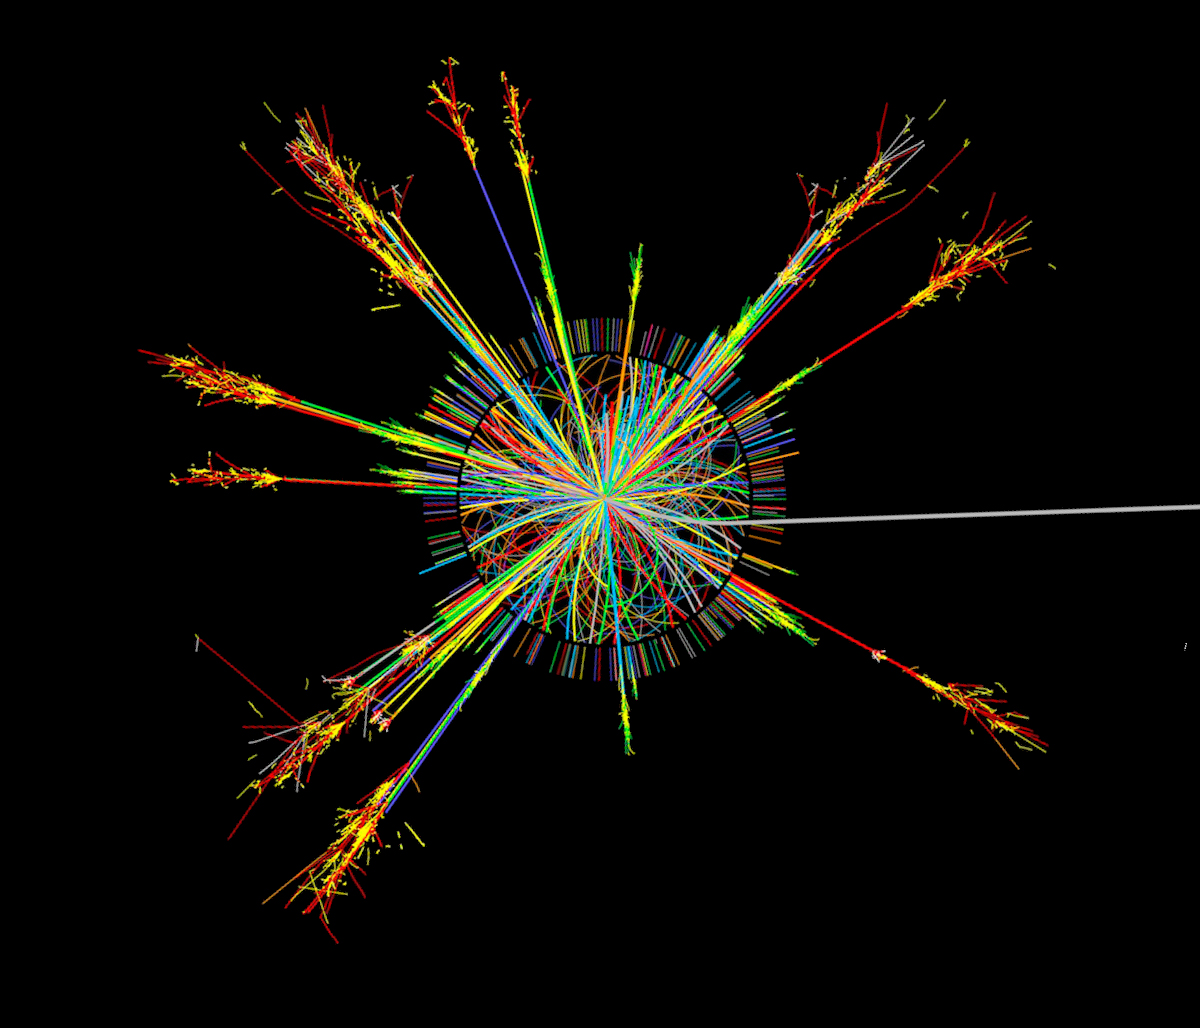
\includegraphics[width=.85\paperwidth]
                        {title/jettitleimage}}
};
\framenode[100pt]{image}
\end{tikzpicture}

% Author
\textcolor{amber}{\subtitlefont{Samuel Alipour-fard}}
\end{center}

\clearpage
\restoregeometry
\setcounter{page}{1}


\ifshowfinalchecks{}
    %%%%%%%%%%%%%%%%%%%%%%%%%%
% Final To-Dos and Checks:
%%%%%%%%%%%%%%%%%%%%%%%%%%
\begin{sambox}{Final Double Checks:}
\begin{itemize}
    \item
    No comments left (\texttt{ctr-f} comment commands);
    
    \item
    No ``\textbackslash iffalse ... \textbackslash fi'' statements or ``...''s.
    
    \item 
    No \texttt{?}s left in citations, references to Sections, etc. (\texttt{ctr-f} `?' in .pdf);
    
    \item
    No files in temp folders;
    
    \item
    Consistency for
    \begin{itemize}
	\item
	high energy (low energy) vs. high-energy (low-energy)
	
	\item
	``nonperturbative'' to ``non-perturbative''

	\item 
	``subjet'' to ``sub-jet''.
	
	\item
	\(\beta\) function \(\to\) beta function (so people can find with ctr-f)
	
	\item
	``plus-function'' to ``plus-distribution''
	
	\item \(d\) to \(\dd\) in integrals
    \end{itemize}
\end{itemize}
\end{sambox}
\fi


%%%%%%%%%%%%%%%%%%%%%%%%%%
% Front Matter:
%%%%%%%%%%%%%%%%%%%%%%%%%%

% ---------------------------------
% Dedication
% ---------------------------------

{\clearpage           % we want a new page
   \thispagestyle{empty}% no header and footer
   \vspace*{\stretch{1}}% some space at the top
   \itshape             % the text is in italics
   \begin{center}
       To the student
   \end{center}
}
{\par % end the paragraph
   \vspace{\stretch{3}} % space at bottom is three times that at the top
   \clearpage           % finish off the page
}


% ---------------------------------
% Other front matter
% ---------------------------------

\section*{Acknowledgements}
\markboth{Acknowledgements}{}


\newpage

\section*{Preface}
\markboth{Preface}{}


% Include a link to the thesis template

First, and most importantly, please remember that problems are a \textit{shortcut} to understanding, not ``something extra''.
%
At least, good problems are :D
%
I've tried to select and invent some good problems for you (and if you have any comments or qualms with any of them, you should feel free to email me) that I hope are representative of
\begin{itemize}
    \item
        the story or ``flavor'' of the material;

    \item
        the physical concepts, and the intuition I have for the material;

    \item
        the mathematics required to do some realistic (albeit simple) computations.\footnote{Even some numerical calcules! See \Sec{}}
\end{itemize}
%
From what I've seen and read, active learning is the quickest and only way.
%
Don't forget!


\newpage

\section*{Prerequisites}
\markboth{Prerequisites}{}

\epigraph{``You earn your right to speculate depending on how much work you do.''}{Barton Zweibach}

In order to understand the technical details of the material in this thesis, I expect that the following prerequisites are necessary (if you can understand them without these prerequisites, great work!):
\begin{itemize}
    \item
        A course in quantum field theory, or at least an understanding of quantum mechanics and the basics of particle physics.

    \item

\end{itemize}

In addition, I expect that you should probably be able to understand the following pieces of physics:
\begin{itemize}
    \item
        The strong coupling \(\alpha_s(\mu)\) obeys the \vocab{renormalization group equation}
        \begin{equation}
        \mu \frac{d}{d\mu} \alpha_s(\mu) = \beta(\alpha_s(\mu))
        =
        - \sum_{n=0}^\infty \beta_n
        {\left(\frac{\alpha_s(\mu)}{4\pi}\right)}^{n+2},
        \end{equation}
        \sam{check} with the first \vocab{beta function coefficient}
        \begin{equation}
            \beta_0
            =
            \frac{1}{4\pi}\le(
                \frac{11}{3} C_A - \frac{4}{3} T_F n_f
            \ri)
            ,
        \end{equation}
        taking an important role at one-loop and in the studies in this thesis.

    \item
        The running of the strong coupling leads to a special scale by \vocab{dimensional transmutation}:
        %
        given the coupling at some scale \(\mu\), the form of the beta function indicates that the coupling becomes infinite at a scale we call \(\LambdaQCD\).
        %
        Ignoring the effects of the beta-function coefficients other than \(\beta_0\), we have
        \begin{equation}
            \LambdaQCD = \mu \exp\left(-\frac{1}{2\beta_0 \alpha_s(\mu)}\right).
        \end{equation}
        \sam{This was just written by copilot -- double check in terms of these definitions.}
\end{itemize}


\newpage

% =====================================
\section*{Notation and Terminology}
% =====================================
\markboth{Notation and Terminology}{}

% =====================================
\begin{sambox}{Resources}{}
    % ---------------------------------
    \begin{itemize}
        \item
            Larkoski Chapter 9:
            %
            ee to hadrons, jets, splitting functions, pheno problems

        \item
            Foundations Chapter 8:
            %
            Factorization, Mellin, DGLAP, sum rules

        \item
            Substructure Chapter 1:
            %
            Substructure motivation
    \end{itemize}
    % ---------------------------------
\end{sambox}
% =====================================

\begin{sambox}{Some TODOs for Sam}{}
    \begin{itemize}
        \item
            Is there a proof that pdfs and fragmentation functions are universal?
            %
            Should put this in somewhere...

        \item
            \sam{Does fragmentation belong in a place where pdfs can fit in..?
                %
                Seems like factorization is the actual important piece. But my thesis is not about factorization!
                %
                I need to find a tasteful way to include it.
            }

        \item
            \sam{Need to fix header on problem pages, which simply use the most recent appendix instead.}
    \end{itemize}
\end{sambox}

Here is some common, and relatively important, notation used throughout this thesis.
%
See \Sec{morenotation} for a more comprehensive list.

\begin{itemize}
    \item
        A \vocab{calcule} is a small calculation, often a simple example or a part of a bigger calculation.

    \item
        \(\eqdelta\) denotes equality by definition;

    \item
        For notational simplicity, I will set the physical constants \(\hbar = c = 1\) in all printed equations;

    \item
        \sam{Metric signature}

    \item
        The Mellin transform of a function \(f(x)\) on the interval $(0,\infty)$ is defined as
        \begin{align}
            \mathcal{M}[f](s)
            \eqdelta
            \int_0^\infty \,\frac{\dd x}{x}\, x^{s-1} \, f(x)
            \eqdelta
            \hat f(s)
            .
        \end{align}

        For all of the applications in this work, other than some derivations which are relegated to the Problems \sam{of Chapter...}, the functions in whose Mellin transforms we are interested will have support only on the interval \((0,1)\).
        %
        Therefore, unless stated otherwise, the Mellin transform appearing in this work will appear in the form
        \begin{align}
            \hat f(s)
            \eqdelta
            \int_0^1 \,\frac{\dd x}{x}\, x^{s-1} \, f(x)
            .
        \end{align}

        \sam{Put into the text where relevant}

        \sam{Mention here the part of the text where this appears and the problems in which it appears}

    \item
        \sam{LO, NLO, LL, NLL, etc.}

    \item
        The \textit{energy fraction} carried by a particular particle in a scattering event or jet, relative to the total energy of the event or jet, will play an important role in this thesis.
        %
        We will use the symbol \(z_i\) to denote the energy fraction particle \(i\) within a jet or event:
        \begin{align}
            z_i
            \eqdelta
            \frac{E_i}{E_\text{tot}}
            .
        \end{align}

    \item
        A useful definition for clarity is that of the value of \(\alpha_s\) divided by \(4\pi\), since this quantity appears in loop computations (which often have a \(4\pi\) suppression):
        \begin{subequations}
        \begin{align}
            a_s = \frac{\alpha_s}{4\pi}
        \end{align}
        \end{subequations}
\end{itemize}


\clearpage

% ---------------------------------
% Table of Contents
% ---------------------------------
\tableofcontents{
    \fancyhead[LO]{\slshape\contentsname}
    \fancyhead[RE]{\slshape\contentsname}
}

\clearpage{}

% ---------------------------------
% List of Figures
% ---------------------------------
\listoffigures{\fancyhead[LE]{\slshape\listfigurename}}
% \clearpage
% \listoftables{\fancyhead[LE]{\slshape\listtablename}}


% %%%%%%%%%%%%%%%%%%%%%%%%%%%%%%%%%%%%
% Chapters:
% %%%%%%%%%%%%%%%%%%%%%%%%%%%%%%%%%%%%

\mainmatter{}

% Chapter titles with numbers
\titleformat{\chapter}[display]
{\normalfont\huge\bfseries\sffamily}{}{25pt}{\chaptitle}
\titlespacing*{\chapter} {0pt}{110pt}{20pt}

% ==============================================
\chapter{Quantum Chromodynamics:\\A Picture Book}

% ==============================================
% The first chapter has no appendices (appendices add new line to toc automatically..?)
% so we add a new toc line manually here
\addnewlinetotoc{}
\clearpage{}

% ==============================================
\chapter{Particles Inside Particles:\\Jets and Jet Substructure}

% ==============================================
\section{The physical picture}
% ==============================================

% -----------------------------------
% Figure Comment:
% -----------------------------------
\begin{figure}[t!]
    % Figure graphics
    \centering
    
\includegraphics[width=\textwidth]{figures/tempfig}

    % Caption
    \caption{
        Caption text
    }

    % Figure Label
    \label{fig:label}
\end{figure}

% -----------------------------------

% ---------------------------------------
\subsection{Splitting Functions}
% ---------------------------------------

% ---------------------------------------
\subsection{Renormalization}
% ---------------------------------------

% ==============================================
\section{Confinement Project?}
% ==============================================


% ==============================================
\section{Jets and Renormalization}
% ==============================================


% ==============================================
\section{Connecting back out}
% ==============================================

% ==============================================
\section*{Chapter Appendix: More on distributions}
% ==============================================

% ---------------------------------------
\subsection{Definitions}
% ---------------------------------------

% ---------------------------------------
\subsection{Derivations}
% ---------------------------------------

% ---------------------------------------
\subsection{Diagrammatica}
% ---------------------------------------


% ==============================================
\section*{Chapter Appendix: Derivation of the splitting functions}
% ==============================================

% ---------------------------------------
\subsection{Picture and Sketch}
% ---------------------------------------

% ---------------------------------------
\subsection{Proof}
% ---------------------------------------


% ==============================================
\section*{Chapter Appendix: Derivation of the DGLAP equations}
% ==============================================

% ---------------------------------------
\subsection{Picture and Sketch}
% ---------------------------------------

% ---------------------------------------
\subsection{Proof}
% ---------------------------------------

% ==============================================

% ==============================================
\chapter[Inside Particles: Jets and Resummation]{Inside Particles:\\Jets and Resummation}
\markboth{\bf Chapter \thechapter: Jets and Resummation}{}

% \markboth{\bf Chapter \thechapter: Jets and the Microscopes of Particle Physics}{}

% ==============================================
\section{The physical picture}
% ==============================================

% -----------------------------------
% Picturebook figure
% -----------------------------------
\reusefigure[ht]{picturebook_jets}


% ---------------------------------------
\subsection{Jets}
% ---------------------------------------
\textbf{What is a \gls{jet}?}

A collective degree of freedom which carries information about a seed parton [sic];
%
experimentally robust, theoretically well-defined, and calculable in perturbation theory.

Sources of noise later.
%
For now, develop intuition/precision about what jets are.

% https://gsalam.web.cern.ch/gsalam/talks/repo/2008-cms-jets.pdf
% Jet (definitions) provide central link between expt., “theory” and theory
% See slide 54+
% Perhaps worth linking with Sterman-Weinberg jets

% https://conference.ippp.dur.ac.uk/event/311/contributions/1403/attachments/1133/1289/jettheory.pdf

% https://www-sciencedirect-com.libproxy.mit.edu/science/article/pii/S014664101600034X?via%3Dihub

\begin{itemize}
    \item
    A common theoretical idea is that a jet is a proxy for a parton that appears in the Lagrangian -- QCD jets are then proxies for the quarks and gluons that appear in the QCD sector of the SM Lagrangian.
    \sam{Cite Sterman-Weinberg, and others?}
    %
    The standard approach to defining jets from this point of view is to use a \vocab{jet algorithm} -- a procedure for grouping particles into jets.
    \samtodo{cohere, cite}

    \item
    Another way of thinking is that a jet is simply collinear enhancement of the energy flow in a scattering event.
    \sam{Cite original Russian papers here?}
    %
    From this point of view, we would say that an event with energy flow \(\mc E\) has a jet at the angle \(\hat n\) if
    \begin{align}
        \lim_{\hat n' \to n}\mc E(\hat n) \mc E(\hat n') &\to \infty
    \end{align}
    \samtodo{not quite -- maybe in some limit because we should account for the fact that there are already delta functions in the energy flow (so maybe we should have an integral) and also that even when integrated this shouldn't be infinite...}
    %
    \sam{Maybe we could say something like ``there's a jet in the region \(\mc R\) if \(\int_{\mc R} \dd\Omega \, \mc E(\hat n) \, \mc E(\hat n + \delta \hat n)\) has some properties...}
\end{itemize}
%
These ways of thinking are similar, and we should probably understand how they are the same and how they are different.

\samtodo{Add cartoons for this}

The former idea seems more closely related to renormalization:
%
a jet is a coarse-grained degree of freedom roughly associated with a quark and its associated collinear radiation.

The latter idea is more amenable to experimental studies, and is also connected to more rigorous CFT methods.


% ---------------------------------------
\subsection{Renormalization}
% ---------------------------------------

If you zoom away from the constituents of a system (or towards them), you're likely to be at a renormalization fixed point.
%
\sam{from a youtube video on renormalization!}
%
\sam{Concept of a snowflake composed of molecules -- an interesting ``fixed point'' with fractal structure... and a snowbank, which is still a fixed point but ``uninteresting''.}

% ---------------------------------------
\subsection{Resummation}
% ---------------------------------------
\textbf{What is resummation?}

\begin{itemize}
    \item
        \sam{Generally, a method to turn (potentially divergent) series expansions into compact expressions};

    \item
        \sam{For us, ...}
\end{itemize}

\sam{Other types of resummation:}


\sam{Want discussion of LL, NLL, etc.}

\sam{Then discussion of MLL}


% ==============================================
\section{Parton Showers: Jets from Successive Splittings}
% ==============================================
\label{sec:partonshower}

\sam{LL ``only''? Active research...}


% ---------------------------------------
\subsection{The Partonic Cascade as a Fractal}
% ---------------------------------------



% ---------------------------------------
\subsection{Partonic Fragmentation}
% ---------------------------------------



% ---------------------------------------
\subsection{Scale Evolution from the Shower Perspective}
% ---------------------------------------

\sam{Scale evolution, more generally DGLAP evolution}

\sam{Derive DGLAP following from fragmentation discussion}

\sam{Sharp connection between parton shower and renormalization?}

% https://browse.arxiv.org/pdf/1407.3272.pdf
% https://indico.cern.ch/event/594287/contributions/2497385/attachments/1427850/2191539/scet_2017_waalewijn.pdf

\sam{External connections/generalizations (maybe in App.)?}
\begin{itemize}
    \item
        \sam{What derivations are of DGLAP evolution?}

    \item
        \sam{Original papers? How do they do it?}

    \item
        \sam{Are there several ways to think about this? Maybe I can explain the punchlines of each way of thinking, present the conclusion of DGLAP/evolution in general, and then present the detailed derivations later?}
\end{itemize}




% ---------------------------------------
\subsection{Anomalous Dimensions}
% ---------------------------------------

\sam{cf previous section}



% ==============================================
\section{Subjets Section}
% ==============================================

\sam{Jets coarse grain degrees of freedom, almost always to obtain an ontologically sound representative of a ``partonic degree of freedom''.}

\sam{We can fine-grain this a bit further by looking at subjets inside a jet... is this useful?}


% ==============================================
\section{Jet Substructure}
% ==============================================

\textbf{What is jet substructure?}

\sam{Want to describe several relevant definitions.}

\begin{itemize}
    \item
        \sam{I want to talk about subjets inside a jet}

    \item
        \sam{I want to talk about energy flow inside a jet}
\end{itemize}


% ==============================================
\section{Connecting back out}
% ==============================================

\sam{Perhaps begin discussing sources of noise or hard-to-understand phenomena occurring inside jets, here and previously?}


% %%%%%%%%%%%%%%%%%%%%%%%%%%%%%%%%%%%%
% Appendices
% %%%%%%%%%%%%%%%%%%%%%%%%%%%%%%%%%%%%
\begin{subappendices}
% ==============================================
\section{More Derivations of Historical Phenomena???}
% ==============================================


% ==============================================
\section{Jet Calculus}
% ==============================================


% ==============================================
\section{Derivation of the DGLAP equations}
% ==============================================

% ---------------------------------------
\subsection{Picture and Sketch}
% ---------------------------------------

% ---------------------------------------
\subsection{Proof}
% ---------------------------------------



% ==============================================
\section{Distributions from Renormalization}
% ==============================================
Splitting functions are weird and come from virtual corrections

\begin{itemize}
    \item
        Yorikiyo Nagashima: Elementary Particle Physics

    \item
        Schwartz
    \item
        Structure of the proton
    \item
        Foundations of pQCD
\end{itemize}

% ---------------------------------------
\subsection{Picture and Sketch}
% ---------------------------------------

% ---------------------------------------
\subsection{Proof}
% ---------------------------------------


\begin{itemize}
    \item
        Amplitudes to splitting functions

    \item
        Others?

    \item
        Virtual quanta (WW and Landau reference?)
\end{itemize}

% ---------------------------------------
\subsection{Sum Rules}
% ---------------------------------------


% ==============================================
\section{More on distributions}
% ==============================================

% ---------------------------------------
\subsection{Definitions}
% ---------------------------------------


% ---------------------------------------
\subsection{Derivations}
% ---------------------------------------

% ---------------------------------------
\subsection{Diagrammatica}
% ---------------------------------------


\end{subappendices}

% %%%%%%%%%%%%%%%%%%%%%%%%%%%%%%%%%%%%
% Problems
% %%%%%%%%%%%%%%%%%%%%%%%%%%%%%%%%%%%%
\begin{problems}

%gsalam link above
\makeprob{IRC Safety: Jet Algorithms}{}{
    Which of the following algorithms for identifying a jet is IRC safe?
    \begin{itemize}
        \item
    \end{itemize}
}



\makeprob{Regimes and Accuracy \sam{better name}}{}{

    \begin{enumerate}
        \item
            Show that LO \(\implies\) \(Q \gg \LambdaQCD\).

        \item
            Argue that \(\LambdaQCD\) can be expressed as a non-perturbative scale.

        \item
            Show that LL \(\implies\) scale for the observable...

    \end{enumerate}
}



\makeprob{No Emission Probability}{}{
    \sam{Problem regarding probability of no emission}


    \begin{enumerate}[label=\roman*)]
        \item
            Between two angles

        \item
            Between two mass scales

         \item
             Between an angle and a mass scale
    \end{enumerate}
}




\makeprob{Fragmentation in a Parton Shower}{}{
    \sam{Problem regarding parton shower evolution}

    \sam{Comparison}
}

\makeprob{Energy Loss of Jet}{}{
    \sam{Problem regarding energy loss of a jet?}
    \sam{Generic splitting function? Try different splitting functions with different physical motivations to check intuition?}

    \sam{Uhhh... perhaps too far}
}

\makeprob{Fragmentation of Partons into Partons}{}{
    % Based on \url{https://www.sciencedirect.com/science/article/pii/0550321378900159}

    In this problem, we use the following notation:
    \begin{itemize}
        \item
            Let mid-Roman letters (\(i,\,j,\,k\)) denote flavors of partons;

        \item
            Let \(\mc P_{j\leftarrow i}(z) \dd z\) denote the probability of finding a parton of flavor \(j\) with momentum fraction between \(z\) and \(z + \dd z\) of the initiating parton \(i\);

        \item
            Let \(a_s\,\,p_{k_1\,k_2 \leftarrow i}(z) \dd z\) denote the probability that a parton of flavor \(i\) splits exactly into two partons with flavors \(k_1\) (with energy fraction between \(z\) and \(z + \dd z\)) and \(k_2\).
            %
            Furthermore, let us abuse notation and define \(\sum_{k'} p_{j\,k' \leftarrow i}(z) \eqdelta p_{j\leftarrow i}(z)\).
    \end{itemize}
    \sam{Move into notation section}

    We will also make the assumption that \(\alpha_s\), and hence \(a_s\), is independent of the energy scale associated with the splitting.


    \begin{enumerate}[label=\roman*)]
        \item
            Argue on physical grounds that
            \begin{align}
                \label{eqn:feynman_field_fragmentation_formula}
                \mc P_{j\leftarrow i}(z)
                &=
                c \delta(1-z) \delta_{ij}
                +
                a_s \, p_{j \leftarrow i}(z)
                +
                a_s \int_z^1 \frac{\dd y'}{y'} \, \sum_{k_1',\,k_2'} \,
                    \mc P_{j\leftarrow k'}(z/y')
                    \,
                    p_{k' \leftarrow i}(y')
                ,
            \end{align}
            and write the associated formula in Mellin space.
            % \begin{align}
            %     \label{eqn:feynman_field_fragmentation_formula_mellin}
            %     \hat {\mc P}_{j\leftarrow i}(n)
            %     &=
            %     a_s
            %     \le(
            %         \hat {p}_{j\leftarrow i}(n)
            %         +
            %         \hat {\mc P}_{j\leftarrow k'}(n)
            %         \,\,
            %         \hat {p}_{k' \leftarrow i}(n)
            %     \ri)
            %     ,
            % \end{align}
            % where we have left the sum on \(k'\) implicit.

            \sam{Need no emission probability}

        \item
            \samtodo{Invert matrix, find moment, invert Mellin}
    \end{enumerate}
}

\makeprob{Fragmentation of Partons into Hadrons}{}{
}


\makeprob{Sum Rules after Renormalization}{}{
    \sam{Problem regarding sum rules after renormalization}
}

\makeprob{Fragmentation of heavy partons}{}{
    \sam{
    %\href{https://pdg.lbl.gov/2019/reviews/rpp2019-rev-frag-functions.pdf}
    {PDG} says heavy hadrons more hard... could be fun to solve with those initial conditions and compare to data}
}

\end{problems}

% ==============================================

% ==============================================
\chapter[Removing the Rubble: Grooming and Cleanup Fish]{Removing the Rubble:\\Grooming and Cleanup Fish}
\markboth{\bf Chapter \thechapter: Grooming and Cleanup Fish}{}

% ==============================================
\section{The physical picture}
% ==============================================

% -----------------------------------
% Picturebook figure
% -----------------------------------
\reusefigure[ht]{picturebook_substructure}


% ==============================================
\section{Jet Substructure}
% ==============================================

% ==============================================
\section{Jets, Data, and Noise}
% ==============================================

Sources of noise:

\begin{itemize}
    \item
        Hadronization \(\to\) pdfs and ffs
    \item
        ``Track noise'': detector effects \(\to\) track functions

    \item
        UE from multiple pp interactions (pomerons, etc.?)
    \item
        Pileup (less theory, large \(N\))
\end{itemize}

Nice thing about grooming: control over many sources of low energy contamination at once!

% ---------------------------------------
\subsection{Jet Grooming and Pileup Mitigation}
% ---------------------------------------



% ==============================================
\section{Pileup and Infrared Annihilation (PIRANHA): A paradigm for continuous jet grooming}
% ==============================================

% ---------------------------------------
\subsection{Continuity as a bridge between grooming and pileup mitigation}
% ---------------------------------------


% ---------------------------------------
\subsection{More PIRANHA}
% ---------------------------------------

% ==============================================
\section{Connecting back out}
% ==============================================


% %%%%%%%%%%%%%%%%%%%%%%%%%%%%%%%%%%%%
% Appendices
% %%%%%%%%%%%%%%%%%%%%%%%%%%%%%%%%%%%%
\begin{subappendices}

% ==============================================
\section{Derivations}
% ==============================================


% ==============================================
\section{Feeding Frenzy}
% ==============================================


\end{subappendices}


% %%%%%%%%%%%%%%%%%%%%%%%%%%%%%%%%%%%%
% Problems
% %%%%%%%%%%%%%%%%%%%%%%%%%%%%%%%%%%%%
\begin{problems}
\begin{problem}
    Test Problem
\end{problem}
\end{problems}

% ==============================================

% ==============================================
\chapter{Reconstructing the Rubble:\\Event Shapes and Weighted Correlators}

% ==============================================
\section{The physical picture}
% ==============================================

% -----------------------------------
% Figure Comment:
% -----------------------------------
\begin{figure}[t!]
    % Figure graphics
    \centering
    
\includegraphics[width=\textwidth]{figures/tempfig}

    % Caption
    \caption{
        Caption text
    }

    % Figure Label
    \label{fig:label}
\end{figure}

% ==============================================


% =====================================
% Discussion and Conclusions:
% =====================================
% Avoiding unwanted blank pages between chapters
\begingroup{}
\renewcommand{\cleardoublepage}{}
\renewcommand{\clearpage}{}

% ==============================================
% ==============================================
\chapter{Conclusions}
% ==============================================
\markboth{\small \textsc{Chapter \thechapter}: \bf Conclusions}{}
\label{sec:Conclusions}

\epigraph{
    \textit{Ignoramus et ignorabimus}

    [We do not know and we will not know]
}{
    Maxim on the limits of knowledge
}

\epigraph{
    \textit{Wir m\"ussen wissen -- wir werden wissen}.
    %
    [We must know -- we will know.]
}{
    \href{smith-at-sfsu.net/Documents/HilbertRadio/HilbertRadio.mp3}{David Hilbert, in response}
}

\epigraph{
    Do not condescend to ask:
    %
    ``Shall we conquer? Shall we be conquered?''
    %
    Fight on!
}{
    Nikos Kazantzakis
}

In this thesis, we studied perturbative manifestations and phenomenological probes of quantum chromodynamics (\gls{qcd}) in particle collisions.
%
After discussing the how quarks and gluons are the building blocks of the vast majority of our visible universe and the basics of \vocab{partonic scattering} in \Chap{particles} and the \vocab{partonic cascade model} for jet formation and substructure in \Chap{jets}, we realized that the real world presented greater challenges.
%
In particular, we understood that tests of our parton-level predictions of perturbative \gls{qcd} (\gls{pqcd}) require us to overcome the presence of \vocab{low-energy pollution}:
%
\gls{hadronization} and \gls{deteffects} (soft distortions) as well as the \glslink{ue}{underlying event} and \glslink{pileup}{pileup} (additive contamination).
%
With the tools of \gls{pqcd} honed in our introductory chapters, we undertook the task of \vocab{\gls{jet-grooming}} in \Chap{grooming}, where we explicitly removed soft radiation from jets in order to access high-energy, pollution-free degrees of freedom.
%
We began by building intuition for traditional hard-cutoff methods for grooming before building the framework of \PIRANHA{} for continuous grooming and showcasing its formal and phenomenological strengths.
%
Finally, in \Chap{ewocs}, we explored the techniques of \vocab{energy-weighted correlation functions}, with the goal of \textit{ignoring} the low-energy effects of pollution through energy weighting.
%
We introduced the basic theory of the energy-energy correlator (\gls{eec}) for probing angular correlations in collision events, discussed its efficient and visually intuitive higher point generalizations, and even initiated the study of \vocab{energy-weighted observable correlations} (\glspl{ewoc}) to probe arbitrary non-angular correlations, such as the pair-wise masses of subjets.


It has been a privilege to explore the universe with you.
%
Our goal has been to develop realistic tools for the study of the most fundamental features of our universe that humanity has been able to experimentally probe.
%
Our method was to develop collider observables whose behavior illuminates the structure of \gls{qcd} even through the obfuscating haze of contamination generated both by theoretical and experimental effects.
%
As stated by Andrew Larkoski, ``the art of jet substructure... is in the construction of observables'' \cite{}.
%
With the impressionist exposition and few new brush strokes presented in this thesis, we hope we have been able to share our sincere appreciation of the arts of jet substructure and quantum field theory.
%
A more precise understanding of the tools we presented here will require further, finer brush strokes:
%
precision calculations, experimental measurements, the modelling of theoretical and experimental uncertainties, and beyond.
%
But those tales are for another day, and another teller.

% ==============================================
% No appendices, so again we add a new toc line manually
\addnewlinetotoc{}
\newpage{}
\endgroup{}


% %%%%%%%%%%%%%%%%%%%%%%%%%%%%%%%%%%%%
% Appendices
% %%%%%%%%%%%%%%%%%%%%%%%%%%%%%%%%%%%%

\begin{appendices}

% ==============================================
\chapter{More Notation and Terminology}
% ==============================================
\markboth{More Notation and Terminology}{}

\sam{Thinking it might be useful to have a place to stick more detailed terminology and less detailed terminology}.
\end{appendices}



% %%%%%%%%%%%%%%%%%%%%%%%%%%%%%%%%%%%%
% Back Matter
% %%%%%%%%%%%%%%%%%%%%%%%%%%%%%%%%%%%%

\backmatter{}

% Chapter titles without numbers
\titleformat{\chapter}[display]
{\normalfont\huge\bfseries\sffamily}{}{25pt}{\chaptitlenonumber}
\titlespacing*{\chapter} {0pt}{110pt}{20pt}

\chapter[\bf Bonus Problems]{Bonus Problems}
\markboth{\bf Bonus Problems}{}
% =====================================
\section*{Mellin Transforms}

\begin{sambox}{Some resources}{}
% https://users.dimi.uniud.it/~giacomo.dellariccia/Glossary/transforms/Oosthuisen2011.pdf

    \href{https://users.dimi.uniud.it/~giacomo.dellariccia/Glossary/transforms/Bertrand\%20J.Bertrand\%20P.Ovarle.2000.pdf}{Bertrand, Ovarlez, 2000}

    \href{https://en.wikipedia.org/wiki/Integral_transform}{Wikipedia: Integral Transform}

    \href{https://en.wikipedia.org/wiki/Fourier_transform_on_finite_groups}{Fourier transform on finite groups}

    \href{https://mathoverflow.net/questions/79868/what-does-mellin-inversion-really-mean}{MathOverflow: What does Mellin inversion really mean?}

    \href{https://people.cs.uchicago.edu/~laci/reu02/fourier.pdf}{The Fourier Transform and Equations over Finite Abelian Groups}

    \href{https://golem.ph.utexas.edu/category/2010/11/integral_transforms_and_pullpu.html}{Integral Transforms and the Pull-Push Perspective, I}

    \href{https://en.wikipedia.org/wiki/Inverse_scattering_transform}{Inverse scattering transform (Nonlinear generalizations)}

    \href{https://en.wikipedia.org/wiki/Schwartz_kernel_theorem}{Schwartz kernel theorem}

    \href{https://math.stackexchange.com/questions/501899/importance-of-schwartz-kernel-theorem}{Math StackExchange: Importance of Schwartz kernel theorem}

    \href{https://math.stackexchange.com/questions/2623515/schwartz-kernel-theorem-and-dual-topologies}{Math StackExchange: Schwartz kernel theorem and dual topologies}

    \vspace{.5em}

    \textbf{Applications?}

    \href{https://watermark.silverchair.com/748_1_online.pdf?token=AQECAHi208BE49Ooan9kkhW_Ercy7Dm3ZL_9Cf3qfKAc485ysgAABWswggVnBgkqhkiG9w0BBwagggVYMIIFVAIBADCCBU0GCSqGSIb3DQEHATAeBglghkgBZQMEAS4wEQQMp8SxgPn6c7OBLlGhAgEQgIIFHmy00C8eTOUHPbWo8YSihdv0C7NlSfT03xtgMgSAn8fZC5ht3MMECj9-CC6UPP0eJmNWuIgvSj0GaqPDlIC5_WCruiOyqTClvbnr3yPMmV50MYWekQ-cr2ZXoQPJHc2bnnB1DEPxsEaO_PvF5u_2pE4jjqf0CG4JGhHVLPyEpciWGpE1Kh5AlOVxGqy7d7OoL73SJ5obxDW0VztTBhEHp8Z2UDNqGx9beHfyjs62oaMZrdIxAW-zO2UeC53xm1YK-o42GA4WVxeNJndfcHgO-Div8Aa0wSAZc928-vtnhb2sEep9kAGB0lf8a_VCWdY5oCbvS5R1Qls0kuNpdIwLzRo5jM7XBiX1G0hOGzjSPYfvlhlh-xSOP9l17TJ8r1uGyBK4yukjK1SBBkMx67uE3oAzHrMNNx1L1Y6KzYdHeBZQqHB_uB23XbICWBcjfG1Q0U4Esk0MLqMwCL7FvfR25qlfDyDBgypeKopm80aC16fyFdgxtYs7M_bvit4-UK-0dhJGek9ROuQWueXdiThX7MnlWoZ2680UmF49sl5SLlqccH4AGFEEa3LHYVkeUlG6cJhVBmLXBCFpLJm2hcV7spbzEp8RMihe1yAo75YlCnVPNMfSHIggSEatpaYnSFYb5XymdnD1oWj4mQu7DVjnyNi3nzpxGq9Wm0yRXleWhNUMjg-BYQHUe6m2DZ2-zp3sHrvCEywoTOob054ONhNlXbQfwzFyTZrZQ5UtI9UIfb-tRm9FknCpMu9r6FtBT--OYfbNU7pf7d2Vf2YSKu3UmwQ6yyyc_h6qXB4dHdPMnyGKN0rIvw0rJ_KK_qkTwNeEUkwuIltITMCW9UwVchCXjFqpCOf32Ag5N8383O1jBaOEeswn4wz9DH0b1qQW5304289zPqddB6BmsCqP-y7Z-iq-0gjif7e-gjuyBxqIm9OuW90lZqdzkZS8uElGHlYHRseRetE09YqoLzEwBzAv1Xa2vqx0L8NkXOUQdYQGlrR1bk_Bmim7WsPpGwcirDUgb_NMnV5exHa8xPcgpEH5NGiOTbIbaxiCa8j9-1ULa-ds_-vLGAJhT3PA32wfkI2zwtlfCg-fMuvzDFOfFOy0eMkXS3CDd8cRNeLbdXOqc43wSs9Vj3lVWzP-PDYI_zX44fXkpFKAVdv1GAYRnZrCg36rR-Af8yNr7X_9MnbaJH2t05hKPTQsRERXRTtOHFe5kNaliQevn2LmoJEI4D7Kp4htw_kRoTDVsmTe4hRbPuHL0xHMH8si0OH6_l1ji_WM5IfLR6tImH5-7hcF_EizivLaxAAcEXfQ0JEvoR1-kVzqErfrV2CxDhkOMYb3QkJHLxVOCIMfEmTngkzD2Xtm1QDD-i7yd6Oyba1UH4ODMIxm5eFVLBT6s3FV3D5qYDCmwhWftns93iz135CcrvWkuWaTGaGK3NyAYwIe_Z5WuG2MeTwKD6ILw8N6iJ0WB4icc5mf9OBeb3FCXGgW6W_H80nFxTFEP4Dk-cRWGLPgMyIDxpNVgupWdj7qT-0bCGGRzfKxPEU05bx3Io_uTzWEwCeapvu_4eWK9AddxzOLGtkvkr0O3m34_8QvD-ww-VilIdoXe189dBVRb1g3knDQHbt59Yqq1LKZwvcH9Zr9JE49qN1xyFJZnbsIGaYzHPOrw6pgVfoatpOIzTtivOfdGw6SfeKc9rwUReNp7az0xPBPe7TrH-nNuycvDM-a5klPwcG8dc2rDcb9gaSyN3DP}%
    {The power spectrum of the Mellin transformation with applications to scaling of physical quantities}

    \href{https://phsites.technion.ac.il/eric/wp-content/uploads/sites/6/2019/02/Ariane_Soret_MSc_Thesis.pdf}{Quantum dynamics for a fractal spectrum (thesis)}

    \href{https://www.ncbi.nlm.nih.gov/pmc/articles/PMC3222220/}{A Biologically Plausible Transform for Visual Recognition that is Invariant to Translation, Scale, and Rotation}
\end{sambox}




\makebonusprob{What is the Mellin Transform?}{mellinintro}{
    \sam{Problem regarding Mellin transforms}

    \sam{Check signs and prove}

    \textbf{Warmup by Analogy: Fourier Transform}

    In the Fourier transform, a central role is played by the \emph{translations}
    \begin{align}
        x \mapsto x + a
        .
    \end{align}
    The Fourier transform of a function \(f(x)\) divides the function \(f(x)\) into ``plane-wave'' components which are eigenstates of translation.

    The Fourier transform of a function \(f(x)\) is defined as
    \begin{align}
        \mc F[f(x)](k)
        \eqdelta
        \tilde f(k)
        &\eqdelta
        \int_{-\infty}^{\infty} \dd x \, e^{-ikx} f(x)
        .
    \end{align}

    \begin{enumerate}[label=\roman*)]
        \item
            What is the differential operator \(\mc T\) which implements an infinitesimal translation in \(x\)?
            %
            In particular, we are looking for \(\mc T\) such that:
            \begin{align}
                f(x) + \delta x \, \mc T f(x) = f(x+\delta x)
                .
            \end{align}

        \item
            Argue that the Fourier transform of \(f(x)\) can be divided into three conceptually distinct pieces:
            \begin{itemize}
                \item
                    Integration against a translation-invariant measure;

                \item
                    An eigenstate of the translation operator;

                \item
                    The function \(f(x)\) itself.
            \end{itemize}

        \item
            Using the invariance of the integration measure under translations, show that the Fourier tranform of \(f(x)\) after translation by \(a\) is simply related to the Fourier transform of \(f(x)\):
            \begin{align}
                \mc F[f(x+a)](k) = e^{ika} \tilde f(k)
                .
            \end{align}

        \item
            Show that the Fourier transform of \(\mc T f(x)\) is simply related to the Fourier transform of \(f(x)\).
    \end{enumerate}

    \vspace{.5cm}

    \textbf{Finally: Mellin Transform}

    The Mellin transform is similar to the Fourier transform, except that it is now \emph{dilations} which play a central role:
    \begin{align}
        x \mapsto \lambda x
        .
    \end{align}
    The Mellin transform of a function \(f(x)\) divides the function \(f(x)\) into analogous components which are eigenstates of dilation.

    The Mellin transform of a function \(f(x)\) was defined in \Def{mellin}, and takes the form
    \begin{align}
        \mc M[f(x)](s)
        \eqdelta
        \hat f(s)
        &\eqdelta
        \int_0^\infty \dd x \, x^{s-1} f(x)
        .
    \end{align}

    \begin{enumerate}[label=\roman*)]
        \item
            What is the differential operator \(\mc D\) which implements an infinitesimal \vocab{dilation} in \(x\)?
            %
            In particular, we are looking for \(\mc D\) such that:
            \begin{align}
                f(x) + \delta \lambda \, \mc D f(x)
                =
                f\le(\le(1 + \delta \lambda\ri)x\ri)
                .
            \end{align}

        \item
            Argue that the Mellin transform of \(f(x)\) can be divided into three conceptually distinct pieces:
            \begin{itemize}
                \item
                    Integration against a dilation-invariant measure;

                \item
                    An eigenstate of the dilation operator;

                \item
                    The function \(f(x)\) itself.
            \end{itemize}

        \item
            Using the invariance of the integration measure under dilations, show that the Mellin tranform of \(f(x)\) after dilation by \(\lambda\) is simply related to the Mellin transform of \(f(x)\):
            \begin{align}
                \mc M[f(\lambda x)](s) = \lambda^{-s} \hat f(s)
                .
            \end{align}
    \end{enumerate}
}



\makebonusprob{Mellin Convolution Theorem}{mellinconvolution}{
    As you will now show, the Mellin transform of two functions can be naturally associated with a convolution of the form
    \begin{align}
        (f \mellinconvolution g)(x)
        =
        \int_0^\infty \frac{\dd y}{y}\, f(y) g(x/y)
        .
    \end{align}

    Prove that the Mellin transform of a convolution of two functions is the product of the Mellin transforms of the individual functions:
    \begin{align}
        \mathcal{M}[f \mellinconvolution g](s)
        =
        \mathcal{M}[f](s) \, \mathcal{M}[g](s)
        .
    \end{align}
    This result will be important in understanding how \sam{certain quantities interact with the DGLAP evolution equations}, and \sam{we can create some physical intuition for this result in the following problem.}

    \sam{State the theorem when applied on functions only with support from 0 to 1}

    \sam{Still want to figure out what exactly is happening here (intuition) -- in diagonalization of dilatation and so on}

    \sam{Could be worthwhile to again compare to Fourier}
}

\makebonusprob{Mellin Convolution Theorem II}{mellinconvolution2}{
    There is another type of convolution that can be expressed simply with Mellin transforms.
    %
    Let us consider the new convolution
    \begin{align}
        (f \circ_{\mc M} g)(x)
        =
        \int_0^\infty\,\dd\xi f(x\,\xi) g(\xi)
        .
    \end{align}
    Show that the Mellin transform of this convolution is
    \begin{align}
        \mathcal{M}[f \circ_{\mc M} g](s)
        \,
        =
        \,
        \mathcal{M}[f](s) \, \mathcal{M}[g](1-s)
        .
    \end{align}

    \sam{Where useful? Ever in jets?}

    \sam{State the theorem when applied on functions only with support from 0 to 1}

    \sam{Still want to figure out what exactly is happening here (intuition) -- in diagonalization of dilatation and so on}

    \sam{Could be worthwhile to again compare to Fourier}
}

\sam{Could be worthwhile to start with a simple power law to show scaling}

\makebonusprob{Abstract Examples of Mellin Transforms}{abstractmellin}{
    \sam{introduce \(f(x)\), \(b\)}
    \begin{enumerate}[label=\roman*)]
        \item
            \(x^b f(x)\)

        \item
            \(\frac{\dd}{\dd x} f(x)\)

        \item
            \(\int_0^x f(t) \dd t\)

        \item
            \(f(x^a)\)?
    \end{enumerate}

    \sam{Give intuition... scaling, etc.}
}


\makebonusprob{More Concrete Examples of Mellin Transforms}{concretemellin}{
    Perform the Mellin transforms of the following functions:
    \begin{enumerate}[label=\roman*)]
        \item
            \(x^n\) for \(x \in [0,1]\)

        \item
            \(\frac{1}{1 + x}\)

        \item
            \(e^{-x}\)

        \item
            \(e^{-a x}\) for \(\Re(a) > 0\), and thus \(\sin(k x)\) and \(\cos(k x)\)

        \item
            \(e^{-x^2}\)

        \item
            \(\frac{1}{1 + e^{-x}}\)
     \end{enumerate}

     \sam{Intuition -- compare some of the different examples...}

}


\makebonusprob{Ramanujan's Master Theorem}{ramanujanmastertheorem}{
    \sam{Problem regarding Ramanujan's master theorem}
}

\makebonusprob{Mellin Inversion Theorem}{mellininversion}{
    \sam{Problem regarding Mellin inversion theorem}
    \begin{align}
        f(x)
        =
        \frac{1}{2 \pi\, i}
        \int_{c - i \infty}{c + i\infty}
        \dd s \, x^{-s} \hat f(s)
    \end{align}
    \sam{Note that it's like a continuous analog of a power series}

    \sam{Hint Inverse Laplace and prove}
}

\makebonusprob{Mellin Transform of a Power Law}{mellinpowerlaw}{
    \begin{enumerate}[label=\roman*)]
        \item
            Fixed scaling -- inverse of delta function
    \end{enumerate}

    \sam{Give intuition... scaling, etc.}
}

\makebonusprob{Parseval's Theorem}{mellinparseval}{
    \sam{Problem regarding Parseval's theorem}

    \begin{align}
        \mc M [f(x) g(x)](s)
        =
        \frac{1}{2\pi\,i}
        \int_{c-i\infty}^{c+\infty}
        \dd p \, \hat f(p) \hat g(s-p)
    \end{align}
}

\makebonusprob{Perron's Formula}{perronformula}{
    \sam{Problem regarding Perron's formula}
}

\sam{Perhaps for later -- show that Mellin transform of the definition of a pdf is a local operator}

\sam{Ian mentions the paper 1011.1485}

\sam{I also found 1107.1499}

\textbf{Fractals:}

\sam{Borrowing the following from the thesis resource in the comments above}

\sam{Section 2.4 -- scaling properties}

\sam{Damn I like this thesis, super cool}

% =====================================
\addnewlinetotoc{}
\newpage{}


\chapter[\bf Solutions to Problems]{Solutions to Problems}
\markboth{\bf Solutions to Problems}{}
% =====================================
% ==============================================
\section*{Chapter 2}
% ==============================================

% ==============================================
\section*{Chapter 3}
% ==============================================

\sam{FIGURE OUT LINKS}


% ==============================================
\section*{Bonus Problems}
% ==============================================

% ---------------------------------------
\BonusSoln{mellinconvolution}
% ---------------------------------------
\sam{FIX BOUNDS}

We want to show that
\begin{align*}
    \mc M[f \mellinconvolution g](s) = \mc M[f](s) \mc M[g](s)
    ,
\end{align*}
where
\(
    \mathcal{M}[f](s) = \int_0^\infty \dd x\, x^{s-1} f(x)
    ,
\)
and
\(
    (f(x) \mellinconvolution g(x))(x)
    =
    \int_x^1 \frac{\dd y}{y}\, f(y) g(x/y)
    .
\)


To solve the problem, it is helpful to re-organize the integral associated with the Mellin transform of the convolution of \(f(x)\) and \(g(x)\):
\begin{align*}
    \int_0^\infty \dd x\, x^{s-1}
    \int_0^\infty \,\frac{\dd y}{y}\,
    f(y) g(x/y)
    =
    \int_0^\infty \,\frac{\dd y}{y}
    f(y)
    \int_0^\infty \dd x\,
    x^{s-1} g(x/y)
    =
    \int_0^1 \dd y \, y^{s-1} f(y)
    \int_0^1 \dd z\, z^{s-1} g(z)
    =
    f(s) g(s)
    .
\end{align*}
In the first equality, we have exchanged the two integrals. % and noted that \(x \in (0,1),\, y \in (x,1)\) cuts out the same region of the plane as \(y \in (0, 1),\,x \in (0,y)\). % From when the bounds were from zero to one
%
In the second equality, we have changed variables from \(x\) to \(z = x/y\) and used \(\dd x\, x^n = y^{n+1}\, \dd z\, z^n\).

\qed{}

\sam{Add discussion of what happens when bounds are from 0 to 1}


% ---------------------------------------
\BonusSoln{mellinconvolution2}
% ---------------------------------------
We want to show that
\begin{align*}
    \mc M[f \circ_{\mc M} g](s) = \mc M[f](s) \mc M[g](s)
    ,
\end{align*}
where
\(
    \mathcal{M}[f](s) = \int_0^\infty \,\dd x\, x^{s-1} f(x)
    ,
\)
and
\(
    (f(x) \circ_{\mc M} g(x))(x)
    =
    \int_0^\infty\,\dd\xi f(x\,\xi) g(\xi)
    .
\)


To solve the problem, it is helpful to re-organize the integral associated with the Mellin transform of the convolution of \(f(x)\) and \(g(x)\):
\begin{align*}
    \int_0^\infty \dd x\, x^{s-1}
    \int_0^\infty \, \dd \xi
    f(\xi x) g(\xi)
    =
    \int_0^\infty \, \dd \xi
    \int_0^\infty \dd (\xi x)\, (\xi x)^{s-1}
    \frac{1}{\xi^s}
    f(\xi x) g(\xi)
    =
    \int_0^\infty \, \dd \xi
    \xi^{-s}
    g(\xi)
    \int_0^\infty \dd z\, z^{s-1}
    f(z)
    =
    f(s) g(1-s)
    .
\end{align*}
In the first equality, we have exchanged the two integrals and changed variables from \(x\) to \(\xi x = z\), and in the final equality we have used \(-s = (1-s) - 1\) to note that the first integral is equal to \(g(1-s)\).

\qed{}

% ---------------------------------------
\BonusSoln{abstractmellin}
% ---------------------------------------

\begin{align}
%\label{eq:}
    x^b f(x)
    &\to
    \\
    \frac{\dd}{\dd x} f(x)
    &\to
    \\
    \int_0^x f(t) \dd t
    &\to
    \\
    f(x^a)
    &\to
    \frac{1}{a} \hat f(s/a)
\end{align}

\sam{intuition ffor each}





% ---------------------------------------
\BonusSoln{concretemellin}
% ---------------------------------------


\begin{align}
%\label{eq:}
    x^n
    &\to
    \\
    \frac{1}{1+x}
    &\to
    \beta(s, 1-s)
    =
    \Gamma(s) \Gamma(1-s)
    \\
    e^{-x}
    &\to
    \Gamma(s)
    \\
    e^{-a x}
    &\to
    \Gamma(s) a^{-s}
    \\
    \sin(k x)
    &\to
    \Gamma(s) \sin\left(\frac{\pi s}{2}\right) k^{-s}
    \\
    \cos(k x)
    &\to
    \Gamma(s) \cos\left(\frac{\pi s}{2}\right) k^{-s}
    \\
    e^{-x^2}
    &\to
    \frac{1}{2}\Gamma\le(\frac{s}{2}\ri)
    \\
    \frac{1}{e^{x} - 1}
    &\to
    \Gamma(s)\zeta(s)
    \\
    \frac{1}{e^{x} + 1}
    &\to
    \le(1 - 2^{1-s}\ri)\Gamma(s)\zeta(s)
\end{align}


% ==============================================
\section*{Chapter 4}
% ==============================================


% ==============================================
\section*{Chapter 5}
% ==============================================

% =====================================

\clearpage

% %%%%%%%%%%%%%%%%%%%%%%%%%%%%%%%%%%%%
% Bibliography:
% %%%%%%%%%%%%%%%%%%%%%%%%%%%%%%%%%%%%

% Chapter titles without numbers
\titleformat{\chapter}[display]
{\normalfont\huge\bfseries\sffamily}{}{25pt}{\chaptitlenonumber}
\titlespacing*{\chapter} {0pt}{110pt}{20pt}

% New header
% \renewcommand\bibname{\bf Bibliography}
% DEBUG : is bibliography capitalized in the header?

\bibliography{thesis_bib}


% %%%%%%%%%%%%%%%%%%%%%%%%%%%%%%%%%%%%
% Glossary
% %%%%%%%%%%%%%%%%%%%%%%%%%%%%%%%%%%%%

% Adding all terms to glossary
% (``unused'' means that entries added in this way will not have an associated page number)
\glsaddallunused{}

% Alternative with page number, I can't see ever wanting this though
% \glsaddall{}


% - - - - - - - - - - - - - - - - -
% Acronyms
% - - - - - - - - - - - - - - - - -
% Fixing appearance in TOC
\addnewlinetotoc{}

\printglossary[type=\acronymtype]


% - - - - - - - - - - - - - - - - -
% Glossary
% - - - - - - - - - - - - - - - - -
% Fixing appearance in TOC
\addnewlinetotoc{}

% Removing unwanted newpage
\clearpage
\begingroup\let\newpage\relax
\printglossary
\endgroup


% - - - - - - - - - - - - - - - - -
% Index
% - - - - - - - - - - - - - - - - -
% DEBUG: Do I even want an index?

% Fixing appearance in TOC
\addnewlinetotoc{}

% Removing unwanted newpage
\clearpage
\begingroup\let\newpage\relax
% \printunsrtglossary[type=index,style=bookindex] % index
\printindex
\endgroup

% DEBUG: not sure which command to use to generate index
% \printglossary[type=index,style=bookindex] % index
% \printindex


% TODOs (acronym/glossary/index):
% TODO: See wiki: Dual entries with reference to a glossary entry from an acronym
% TODO: Figure out how to add items to index as well
% See: https://tex.stackexchange.com/a/267345
% TODO: Link EEC and EWOC to Event Shape


% =====================================
% %%%%%%%%%%%%%%%%%%%%%%%%%%%%%%%%%%%%
\end{document}
% %%%%%%%%%%%%%%%%%%%%%%%%%%%%%%%%%%%%
% =====================================
